%%!TEX root = ./marylie.tex
%%--.----1----.----2----.----3----.----4----.----5----.----6----.----7----.-!

\section{Thin Low Order Multipole}
\begin{quotation}
\noindent Type Code:  thlm
\vspace{5mm}

\noindent Required Parameters:
\begin{enumerate}
      \item  BQD (Tesla) \hspace{1em} (normal)
      \item  AQD (Tesla) \hspace{1em} (skew)
      \item  BSEX (Tesla/m) \hspace{1em} (normal)
      \item  ASEX (Tesla/m) \hspace{1em} (skew)
      \item  BOCT (Tesla/$\mbox{m}^2$) \hspace{1em} (normal)
      \item  AOCT (Tesla/$\mbox{m}^2$) \hspace{1em} (skew)
\end{enumerate}

\vspace{5mm}
\noindent Example:
\begin{verbatim}
         octkick    thlm
          0 , 0 , 0 , 0 , 0 , 2.
\end{verbatim}
\end{quotation}
This specifies a map with the user given name {\em octkick}.\index{thin multipole} \index{multipole}  It describes a skew
magnetic octupole, with a path integrated strength of 2 Tesla/$\mbox{m}^2$, in the
kick approximation.

\vspace{5mm}
     Description:
\vspace{2mm}

     The type code {\em thlm} may be used to produce the results of thick
	 multipoles in the limiting case that they become very strong and very
	 short in such a way that the product length times strength approaches a
	 definite limit.  See Exhibit 6.16.1.  Note that the thin low order
	 quadrupole element has no fringe fields.
\newpage
\begin{footnotesize}
\begin{verbatim}
#comment
 Exhibit 6.16.1.
 This is a MARYLIE run illustrating the sign conventions for a
 thin low order multipole.  In this run thin low order multipoles
 are compared with their thick counterparts in limiting cases.
 The beam parameters are those for 800 MeV protons.
#beam
  4.881030646470486
 0.8526309382400936
  1.000000000000000
  1.000000000000000
#menu
 fileout  pmif
   1.00000000000000       12.0000000000000       3.00000000000000
 setzero  zer
  0.000000000000000E+00  1.000000000000000E-08  0.000000000000000E+00
 mapout   ptm
   3.00000000000000       3.00000000000000      0.000000000000000E+00
  0.000000000000000E+00   1.00000000000000
 thqd     thlm
   1.00000000000000      0.000000000000000E+00  0.000000000000000E+00
  0.000000000000000E+00  0.000000000000000E+00  0.000000000000000E+00
 skthqd   thlm
  0.000000000000000E+00   1.00000000000000      0.000000000000000E+00
  0.000000000000000E+00  0.000000000000000E+00  0.000000000000000E+00
 thsex    thlm
  0.000000000000000E+00  0.000000000000000E+00   1.00000000000000
  0.000000000000000E+00  0.000000000000000E+00  0.000000000000000E+00
 skthsex  thlm
  0.000000000000000E+00  0.000000000000000E+00  0.000000000000000E+00
   1.00000000000000      0.000000000000000E+00  0.000000000000000E+00
 thoct    thlm
  0.000000000000000E+00  0.000000000000000E+00  0.000000000000000E+00
  0.000000000000000E+00   1.00000000000000      0.000000000000000E+00
 skthoct  thlm
  0.000000000000000E+00  0.000000000000000E+00  0.000000000000000E+00
  0.000000000000000E+00  0.000000000000000E+00   1.00000000000000
 limqd    quad
  5.000000000000000E-09   200000000.000000      0.000000000000000E+00
  0.000000000000000E+00
 limsex   sext
  5.000000000000000E-10   2000000000.00000
 limoct   octm
  5.000000000000000E-10   2000000000.00000
 arot+q   arot
   45.0000000000000
 arot-q   arot
  -45.0000000000000
 arot+s   arot
   30.0000000000000
 arot-s   arot
  -30.0000000000000
 arot+o   arot
   22.5000000000000
 arot-o   arot
  -22.5000000000000
 clear    iden
 inv      inv
 end      end
#lines
 sklimqd
     1*arot+q      1*limqd       1*arot-q
 sklimsex
     1*arot+s      1*limsex      1*arot-s
 sklimoct
     1*arot+o      1*limoct      1*arot-o
 qdtest
     1*clear       1*limqd       1*inv         1*thqd        1*mapout   &
     1*clear       1*sklimqd     1*inv         1*skthqd      1*mapout
 sextest
     1*clear       1*limsex      1*inv         1*thsex       1*mapout   &
     1*clear       1*sklimsex    1*inv         1*skthsex     1*mapout
 octtest
     1*clear       1*limoct      1*inv         1*thoct       1*mapout   &
     1*clear       1*sklimoct    1*inv         1*skthoct     1*mapout
#lumps
#loops
#labor
    1*fileout
    1*setzero
    1*qdtest
    1*sextest
    1*octtest
    1*end
\end{verbatim}
\end{footnotesize}
Results of qdtest:
\begin{footnotesize}
\begin{verbatim}
matrix for map is :

 1.00000E+00 -5.00000E-09  0.00000E+00  0.00000E+00  0.00000E+00  0.00000E+00
 6.99561E-11  1.00000E+00  0.00000E+00  0.00000E+00  0.00000E+00  0.00000E+00
 0.00000E+00  0.00000E+00  1.00000E+00 -5.00000E-09  0.00000E+00  0.00000E+00
 0.00000E+00  0.00000E+00  6.99547E-11  1.00000E+00  0.00000E+00  0.00000E+00
 0.00000E+00  0.00000E+00  0.00000E+00  0.00000E+00  1.00000E+00 -2.05572E-09
 0.00000E+00  0.00000E+00  0.00000E+00  0.00000E+00  0.00000E+00  1.00000E+00

nonzero elements in generating polynomial are :


matrix for map is :

 1.00000E+00 -5.00000E-09  5.12187E-10 -8.53663E-19  0.00000E+00  0.00000E+00
 6.99554E-11  1.00000E+00 -7.32053E-16 -5.12187E-10  0.00000E+00  0.00000E+00
 5.12187E-10 -8.53663E-19  1.00000E+00 -5.00000E-09  0.00000E+00  0.00000E+00
-7.32053E-16 -5.12187E-10  6.99554E-11  1.00000E+00  0.00000E+00  0.00000E+00
 0.00000E+00  0.00000E+00  0.00000E+00  0.00000E+00  1.00000E+00 -2.05572E-09
 0.00000E+00  0.00000E+00  0.00000E+00  0.00000E+00  0.00000E+00  1.00000E+00

nonzero elements in generating polynomial are :

\end{verbatim}
\end{footnotesize}
Results of sextest:
\begin{footnotesize}
\begin{verbatim}
matrix for map is :

 1.00000E+00 -5.00000E-10  0.00000E+00  0.00000E+00  0.00000E+00  0.00000E+00
 0.00000E+00  1.00000E+00  0.00000E+00  0.00000E+00  0.00000E+00  0.00000E+00
 0.00000E+00  0.00000E+00  1.00000E+00 -5.00000E-10  0.00000E+00  0.00000E+00
 0.00000E+00  0.00000E+00  0.00000E+00  1.00000E+00  0.00000E+00  0.00000E+00
 0.00000E+00  0.00000E+00  0.00000E+00  0.00000E+00  1.00000E+00 -2.05572E-10
 0.00000E+00  0.00000E+00  0.00000E+00  0.00000E+00  0.00000E+00  1.00000E+00

nonzero elements in generating polynomial are :


matrix for map is :

 1.00000E+00 -5.00000E-10  0.00000E+00  0.00000E+00  0.00000E+00  0.00000E+00
 0.00000E+00  1.00000E+00  0.00000E+00  0.00000E+00  0.00000E+00  0.00000E+00
 0.00000E+00  0.00000E+00  1.00000E+00 -5.00000E-10  0.00000E+00  0.00000E+00
 0.00000E+00  0.00000E+00  0.00000E+00  1.00000E+00  0.00000E+00  0.00000E+00
 0.00000E+00  0.00000E+00  0.00000E+00  0.00000E+00  1.00000E+00 -2.05572E-10
 0.00000E+00  0.00000E+00  0.00000E+00  0.00000E+00  0.00000E+00  1.00000E+00

nonzero elements in generating polynomial are :

\end{verbatim}
\end{footnotesize}
Results of octtest:
\begin{footnotesize}
\begin{verbatim}
matrix for map is :

 1.00000E+00 -5.00000E-10  0.00000E+00  0.00000E+00  0.00000E+00  0.00000E+00
 0.00000E+00  1.00000E+00  0.00000E+00  0.00000E+00  0.00000E+00  0.00000E+00
 0.00000E+00  0.00000E+00  1.00000E+00 -5.00000E-10  0.00000E+00  0.00000E+00
 0.00000E+00  0.00000E+00  0.00000E+00  1.00000E+00  0.00000E+00  0.00000E+00
 0.00000E+00  0.00000E+00  0.00000E+00  0.00000E+00  1.00000E+00 -2.05572E-10
 0.00000E+00  0.00000E+00  0.00000E+00  0.00000E+00  0.00000E+00  1.00000E+00

nonzero elements in generating polynomial are :


matrix for map is :

 1.00000E+00 -5.00000E-10  0.00000E+00  0.00000E+00  0.00000E+00  0.00000E+00
 0.00000E+00  1.00000E+00  0.00000E+00  0.00000E+00  0.00000E+00  0.00000E+00
 0.00000E+00  0.00000E+00  1.00000E+00 -5.00000E-10  0.00000E+00  0.00000E+00
 0.00000E+00  0.00000E+00  0.00000E+00  1.00000E+00  0.00000E+00  0.00000E+00
 0.00000E+00  0.00000E+00  0.00000E+00  0.00000E+00  1.00000E+00 -2.05572E-10
 0.00000E+00  0.00000E+00  0.00000E+00  0.00000E+00  0.00000E+00  1.00000E+00

nonzero elements in generating polynomial are :
\end{verbatim}
\end{footnotesize}
\newpage




\section{``Compressed'' Low Order Multipole}
\begin{quotation}
\noindent Type Code:  cplm
\vspace{5mm}

\noindent Required Parameters:
\begin{enumerate}
      \item  Length of element (m).
      \item  BSEX (path integrated strength,Tesla/m) \hspace{1em} (normal)
      \item  ASEX (path integrated strength,Tesla/m) \hspace{1em} (skew)
      \item  BOCT (path integrated strength,Tesla/$\mbox{m}^2$) \hspace{1em} (normal)
      \item  AOCT (path integrated strength,Tesla/$\mbox{m}^2$) \hspace{1em} (skew)
\end{enumerate}

\vspace{5mm}
\noindent Example:
\begin{verbatim}
         compsex    cplm
         2.0 , 3.5 , 0 , 0 , 0
\end{verbatim}
\end{quotation}
This specifies a map with the user given name {\em compsex}.\index{compressed multipole}
\index{multipole}  It describes a
``compressed'' normal sextupole with an original length of 2 meters, and a
path integrated strength of 3.5 Tesla/m.

\vspace{5mm}
     Description:
\vspace{2mm}

     An Exhibit 6.17.1 illustrates, compressed multipoles are the result of removing two half drifts from thick multipoles.  Compressed multipoles are sometimes useful for adding multipole content to dipoles.

\newpage
\begin{footnotesize}
\begin{verbatim}
#comment
 Exhibit 6.17.1.
 This is a MARYLIE run illustrating the sign conventions for
 compressed low order multipoles.  Consider a thick multipole
 of length L.  Then a compressed multipole is gotten by removing
 two half drifts from the thick multipole.  This is done by
 sandwiching the thick multipole between two half drifts with
 negative lengths.  Thus, a compressed multipole is defined by
 the rule

 (compressed multipole) = drift(-L/2) * (thick multipole) * drift(-L/2).

 Conversely, one has the result

 (thick multipole) = drift(+L/2) * (compressed multipole) * drift(+L/2).

 This is verified below for various cases.
 The beam parameters are those for 800 MeV protons.
#beam
  4.881030646470486
 0.8526309382400936
  1.000000000000000
  1.000000000000000
#menu
 fileout  pmif
   1.00000000000000       12.0000000000000       3.00000000000000
 setzero  zer
  0.000000000000000E+00  1.000000000000000E-10  0.000000000000000E+00
 mapout   ptm
   3.00000000000000       3.00000000000000      0.000000000000000E+00
  0.000000000000000E+00   1.00000000000000
 nhdr     drft
  -1.00000000000000
 cpsex    cplm
   2.00000000000000       3.50000000000000      0.000000000000000E+00
  0.000000000000000E+00  0.000000000000000E+00
 skcpsex  cplm
   2.00000000000000      0.000000000000000E+00   3.50000000000000
  0.000000000000000E+00  0.000000000000000E+00
 cpoct    cplm
   2.00000000000000      0.000000000000000E+00  0.000000000000000E+00
   3.50000000000000      0.000000000000000E+00
 skcpoct  cplm
   2.00000000000000      0.000000000000000E+00  0.000000000000000E+00
  0.000000000000000E+00   3.50000000000000
 sex      sext
   2.00000000000000       1.75000000000000
 oct      octm
   2.00000000000000       1.75000000000000
 arot+s   arot
   30.0000000000000
 arot-s   arot
  -30.0000000000000
 arot+o   arot
   22.5000000000000
 arot-o   arot
  -22.5000000000000
 clear    iden
 inv      inv
 end      end
#lines
 sdsex
     1*nhdr        1*sex         1*nhdr
 sksdsex
     1*arot+s      1*sdsex       1*arot-s
 sdoct
     1*nhdr        1*oct         1*nhdr
 sksdoct
     1*arot+o      1*sdoct       1*arot-o
 sextest
     1*clear       1*sdsex       1*inv         1*cpsex       1*mapout   &
     1*clear       1*sksdsex     1*inv         1*skcpsex     1*mapout
 octtest
     1*clear       1*sdoct       1*inv         1*cpoct       1*mapout   &
     1*clear       1*sksdoct     1*inv         1*skcpoct     1*mapout
#lumps
#loops
#labor
    1*fileout
    1*setzero
    1*sextest
    1*octtest
    1*end
\end{verbatim}
\end{footnotesize}
Result of sextest
\begin{footnotesize}
\begin{verbatim}
matrix for map is :

 1.00000E+00  0.00000E+00  0.00000E+00  0.00000E+00  0.00000E+00  0.00000E+00
 0.00000E+00  1.00000E+00  0.00000E+00  0.00000E+00  0.00000E+00  0.00000E+00
 0.00000E+00  0.00000E+00  1.00000E+00  0.00000E+00  0.00000E+00  0.00000E+00
 0.00000E+00  0.00000E+00  0.00000E+00  1.00000E+00  0.00000E+00  0.00000E+00
 0.00000E+00  0.00000E+00  0.00000E+00  0.00000E+00  1.00000E+00  0.00000E+00
 0.00000E+00  0.00000E+00  0.00000E+00  0.00000E+00  0.00000E+00  1.00000E+00

nonzero elements in generating polynomial are :


matrix for map is :

 1.00000E+00  0.00000E+00  0.00000E+00  0.00000E+00  0.00000E+00  0.00000E+00
 0.00000E+00  1.00000E+00  0.00000E+00  0.00000E+00  0.00000E+00  0.00000E+00
 0.00000E+00  0.00000E+00  1.00000E+00  0.00000E+00  0.00000E+00  0.00000E+00
 0.00000E+00  0.00000E+00  0.00000E+00  1.00000E+00  0.00000E+00  0.00000E+00
 0.00000E+00  0.00000E+00  0.00000E+00  0.00000E+00  1.00000E+00  0.00000E+00
 0.00000E+00  0.00000E+00  0.00000E+00  0.00000E+00  0.00000E+00  1.00000E+00

nonzero elements in generating polynomial are :

\end{verbatim}
\end{footnotesize}
Result of octtest
\begin{footnotesize}
\begin{verbatim}
matrix for map is :

 1.00000E+00  0.00000E+00  0.00000E+00  0.00000E+00  0.00000E+00  0.00000E+00
 0.00000E+00  1.00000E+00  0.00000E+00  0.00000E+00  0.00000E+00  0.00000E+00
 0.00000E+00  0.00000E+00  1.00000E+00  0.00000E+00  0.00000E+00  0.00000E+00
 0.00000E+00  0.00000E+00  0.00000E+00  1.00000E+00  0.00000E+00  0.00000E+00
 0.00000E+00  0.00000E+00  0.00000E+00  0.00000E+00  1.00000E+00  0.00000E+00
 0.00000E+00  0.00000E+00  0.00000E+00  0.00000E+00  0.00000E+00  1.00000E+00

nonzero elements in generating polynomial are :


matrix for map is :

 1.00000E+00  0.00000E+00  0.00000E+00  0.00000E+00  0.00000E+00  0.00000E+00
 0.00000E+00  1.00000E+00  0.00000E+00  0.00000E+00  0.00000E+00  0.00000E+00
 0.00000E+00  0.00000E+00  1.00000E+00  0.00000E+00  0.00000E+00  0.00000E+00
 0.00000E+00  0.00000E+00  0.00000E+00  1.00000E+00  0.00000E+00  0.00000E+00
 0.00000E+00  0.00000E+00  0.00000E+00  0.00000E+00  1.00000E+00  0.00000E+00
 0.00000E+00  0.00000E+00  0.00000E+00  0.00000E+00  0.00000E+00  1.00000E+00

nonzero elements in generating polynomial are :
\end{verbatim}
\end{footnotesize}

\newpage
\section{J Map}
\begin{quotation}
\noindent Type Code:  jmap
\vspace{5mm}

\noindent Required Parameters:  None
\vspace{5mm}

\noindent     Example:
\begin{verbatim}
         jay    jmap
\end{verbatim}
\end{quotation}
This specifies a command with the user given name {\em jay}.  It produces a
transfer map whose matrix part is $J$, and whose polynomials $f_3$  and $f_4$  are
zero.

\vspace{5mm}
     Description:
\vspace{2mm}

    It is useful to have the Poisson matrix $J$ available for checking and
exploiting the symplectic condition.\index{J matrix} \index{Poisson matrix}  See section 3.5.  When the ordering
\begin{equation}
z = (X , P_x , Y ,  P_y , \tau , P_\tau)
\end{equation}
is employed for the phase-space coordinates, $J$ takes the form

\begin{equation}
J=\left(
\begin{array}{rrrrrr}
 0 & 1 & 0 & 0 & 0 & 0 \\
-1 & 0 & 0 & 0 & 0 & 0 \\
 0 & 0 & 0 & 1 & 0 & 0 \\
 0 & 0 & -1 & 0 & 0 & 0 \\
 0 & 0 & 0 & 0 & 0 & 1 \\
 0 & 0 & 0 & 0 & -1 & 0
 \end{array}
 \right).
\end{equation}

\newpage
\section{Random Elements}
\begin{quotation}
\begin{tabbing}
\noindent     Type Code:  \=r**** where **** is the type code for the corresponding\\
                          \>standard element.
\end{tabbing}
\vspace{5mm}

\noindent     Required Parameters:
\begin{enumerate}
      \item  ISOURCE

             \ = $-J$ (with $J$ an integer from 1 to 9) to take parameters from
             a parameter  \hspace*{1.5em}set associated with the type code {\em psj}.

             \ = NFILE (with NFILE$\geq$1) to read parameters from the file unit NFILE.

      \item  IECHO

             = 0 not to echo back parameter set values.

             = 1 to write parameter set values at the terminal.

             = 2 to write parameter set values on file 12.

             = 3 to write parameter set values at the terminal
			 and on file 12.
\end{enumerate}

\vspace{5mm}
\noindent Example:
\begin{verbatim}
        badsex    rsext
         17          1
\end{verbatim}
\end{quotation}
The above specifies a random sextupole with user given name {\em badsex}.\index{random elements}  The
parameters for this element are to be read from file 17.

\vspace{5mm}
     Description:
\vspace{2mm}

         An idealized lattice generally has a relatively small number of
elements.  However, in a real lattice, every element may be different due
to errors.  Consequently, the description of a large real lattice with
errors requires a large number of parameters.

         The elements of a large lattice may be specified individually in
\#menu by employing individual user specified names and parameter values.
However, it is also possible to read element parameters from auxiliary
external files.  This may be done for most beam line elements by using the
corresponding {\em random type code mnemonic}.  Random type code mnemonics are
obtained by prefixing the corresponding standard type code mnemonic by the
letter {\em r}.  Listed below are the standard and random mnemonics for elements
having this feature:
\newpage

\begin{center}
\begin{tabular}{ll}
\multicolumn{1}{c}{Standard Mnemonic} &
\multicolumn{1}{c}{Random Mnemonic} \\
\hspace{4em}arot                 &\hspace{3em}rarot \\
\hspace{4em}cfbd                 &\hspace{3em}rcfbd \\
\hspace{4em}cfqd                 &\hspace{3em}rcfqd \\
\hspace{4em}cfrn                 &\hspace{3em}rcfrn \\
\hspace{4em}cplm                 &\hspace{3em}rcplm \\
\hspace{4em}dism                 &\hspace{3em}rdism \\
\hspace{4em}dp                   &\hspace{3em}none  \\
\hspace{4em}drft                 &\hspace{3em}rdrft \\
\hspace{4em}frng                 &\hspace{3em}rfrng \\
\hspace{4em}gbdy                 &\hspace{3em}rgbdy \\
\hspace{4em}gbnd                 &\hspace{3em}rgbnd \\
\hspace{4em}jmap                 &\hspace{3em}none  \\
\hspace{4em}mark                 &\hspace{3em}none  \\
\hspace{4em}nbnd                 &\hspace{3em}rnbnd \\
\hspace{4em}octe                 &\hspace{3em}rocte \\
\hspace{4em}octm                 &\hspace{3em}roctm \\
\hspace{4em}pbnd                 &\hspace{3em}rpbnd \\
\hspace{4em}prot                 &\hspace{3em}rprot \\
\hspace{4em}quad                 &\hspace{3em}rquad \\
\hspace{4em}recm                 &\hspace{3em}rrecm \\
\hspace{4em}sext                 &\hspace{3em}rsext \\
\hspace{4em}sol                  &\hspace{3em}rsol  \\
\hspace{4em}spce                 &\hspace{3em}rspce \\
\hspace{4em}srfc                 &\hspace{3em}rsrfc \\
\hspace{4em}thlm                 &\hspace{3em}rthlm \\
\hspace{4em}twsm                 &\hspace{3em}rtwsm \\
\hspace{2.5em}usr1\ldots  usr20     &\hspace{1.5em}rusr1\ldots rusr20
\end{tabular}
\end{center}
\vspace{5mm}

         A random element is described by giving a user specified name and
random type code mnemonic on one line followed by the number of a parameter
data file on a second line.  See the example below:
\begin{quotation}
\begin{verbatim}
        badsex    rsext
           17        1
\end{verbatim}
\end{quotation}
This describes a random sextupole with user specified name {\em badsex}.  Each
time \Mary makes use of this element, it will read file 17 to obtain the
corresponding set of required parameter values.  The format of the
parameter data file should be the same as the parameter format for a
standard element. In this case (see section 6.10), file 17 should contain a
list of the form shown below:
\[\begin{array}{ccc}
         .50 & , & 3.5 \\
         .49 & , & 3.7 \\
         .51 & , & 3.8 \\
      \vdots &   & \vdots
\end{array}\]
The first number in each line is a sextupole length, and the second is a
sextupole strength.  Note that file 17 is read (without rewinding) each
time the element {\em badsex } is used.  Thus, the user must be careful to be sure
that successive lines in file 17 occur in the order in which they are
needed.

         If desired, use may be made of several parameter data files
simultaneously.  Thus, for example, random quadrupole strengths might be
stored in file 19.  See section 4.2.  The menu could then contain an entry
of the form shown below:
\begin{quotation}
\begin{verbatim}
        badquad    rquad
           19         1
\end{verbatim}
\end{quotation}
This defines a random quadrupole with the user specified name {\em badquad}.  In
this case (see section 6.10), file 19 should contain a list of the form
\[\begin{array}{ccccccc}
         .50 & , & 1.92 & , & 1 & , & 1 \\
         .51 & , & 1.93 & , & 1 & , & 1 \\
         .51 & , & 1.91 & , & 1 & , & 1 \\
\vdots & & \vdots & & \vdots & & \vdots
\end{array}\]
Here the first number in each line is a quadrupole length, the second is a
quadrupole strength, and the remaining 1,1 indicate that each quadrupole
has leading and trailing hard-edge fringe fields.

         \Mary may come to the end of a random parameter file, such as
file 17, during the course of a run.  This could occur, for example, in a
tracking run with a {\em loop}.  When this happens, \Mary rewinds the random
parameter file and resumes reading from the beginning.

Upon occasion it may be useful to draw the parameters for an element from
a parameter set.  See section 7.25.  For example, one may wish to tie the
parameter values of various elements together.  This can be done by
taking their parameter values from a common parameter set.  Note that, if
desired, these common parameter values can be obtained from a random list
on some file.  See section 7.26.  The example below shows the use of a
parameter set:
\begin{quotation}
\begin{verbatim}
        badpar      ps3
         .50   3.5   0 0 0 0
\end{verbatim}
\end{quotation}
\begin{quotation}
\begin{verbatim}
        badsex      rsext
            -3           1
\end{verbatim}
\end{quotation}
This example describes a random sextupole with user specified name {\em
badsex}.  Each time \Mary makes use of this element, it will look at
parameter set 3 to obtain the needed parameter values, which in this case
are .50 for the length and 3.5 for the strength.  Note that the command
{\em badpar} must be invoked in \#labor before {\em badsex} is used in
order for these parameter values to be initialized.  Note also that, to
fulfill format requirements, the parameter set must have six parameter
values even though, in this case, only the first two are used.

\newpage

\section{User Specified Subroutine that acts on phase space data}
\begin{quotation}
\noindent Type Code:  usr1, usr2, $\cdots$ usr10
\vspace{5mm}

\noindent Required Parameters:
\begin{enumerate}
      \item  P1
      \item  P2
      \item  P3
      \item  P4
      \item  P5
      \item  P6
\end{enumerate}

\vspace{5mm}
\noindent Example:
\begin{verbatim}
         foil    usr1
         .1 , .2 , .8 , 0 , 0 , 0
\end{verbatim}
\end{quotation}
This specifies a user written subroutine with the user given name {\em foil}.\index{user specified subroutine}  It
is to do its calculations using the parameter values .1, .2, .8, 0, 0, 0.

\vspace{5mm}
     Description:
\vspace{2mm}

         To be documented by user.  Shown below is the place where the
		 user can put his/her own code in user1.  The include file rays.inc
		 specifies the array where phase space data is stored.  The parameters
		 P1 through P6 are available for the user to employ, and can be varied
		 by the {\em vary} command in connection with fitting and optimization
		 routines.  See section 9.6.

\begin{verbatim}
       subroutine user1(p)
c
c This subroutine .....
c
      include 'impli.inc'
      include 'files.inc'
      include 'rays.inc'
      include 'parset.inc'
c
      dimension p(6)
c
c User supplied code goes here.
c
      return
      end
\end{verbatim}

\newpage



\section{User Specified Subroutine that produces or acts on a map}
\begin{quotation}
\noindent Type Code:  usr11, usr12, $\cdots$ usr20

\vspace{5mm}

\noindent Required Parameters
\begin{enumerate}
      \item  P1
      \item  P2
      \item  P3
      \item  P4
      \item  P5
      \item  P6
\end{enumerate}

\vspace{5mm}
\noindent     Example:
\begin{verbatim}
         mymap    usr11
          1 , 1 , 0 , 0 , 0 , 0
\end{verbatim}
\end{quotation}
This specifies a user written subroutine with the user given name {\em mymap}.\index{user specified subroutine}
It is to do its calculations using the parameters values 1, 1, 0, 0, 0, 0.

\vspace{5mm}
     Description:
\vspace{2mm}

       To be documented by user.  Shown below is the place where the
		 user can put his/her own code in user11.  The calling arrays fa and fm
		 contain the current transfer map.  The parameters
		 P1 through P6 are available for the user to employ, and can be varied
		 by the {\em vary} command in connection with fitting and optimization
		 routines.  See section 9.6.

\begin{verbatim}
      subroutine user11(p,fa,fm)
c
c  This subroutine ....
c
      include 'impli.inc'
      include 'usrdat.inc'
      include 'mldex.inc'
c
      dimension p(6)
      dimension fa(*), fm(6,6)
c
c User supplied code goes here.
c
      return
      end
\end{verbatim}


\newpage



\section{Dispersion Matrix}
\begin{quotation}
\noindent Type Code:  dism
\vspace{5mm}

\noindent Required Parameters:
\begin{enumerate}
      \item  $R_{16}$
      \item  $R_{26}$
      \item  $R_{36}$
      \item  $R_{46}$
      \item  $R_{56}$
\end{enumerate}

\vspace{5mm}
\noindent Example:
\begin{verbatim}
         dismat   dism
          .1 , .2 , 0 , 0 , 0
\end{verbatim}
\end{quotation}
The above specifies a map with user given name {\em dismat}.\index{dispersion matrix}  The diagonal entries of the matrix part $R$ are 1.  The off diagonal entries $R_{16}$ and $R_{26}$ have the values .1 and .2, respectively.  The map has no nonlinear part.

\vspace{5mm}
     Description:
\vspace{2mm}

     This type code produces a linear map with matrix part
\begin{equation}
R=\left( \begin{array}{cccccc}
1 & 0 & 0 & 0 & 0 & R_{16} \\
0 & 1 & 0 & 0 & 0 & R_{26} \\
0 & 0 & 1 & 0 & 0 & R_{36} \\
0 & 0 & 0 & 1 & 0 & R_{46} \\
-R_{26} & R_{16} & -R_{46} & R_{36} & 1 & R_{56} \\
0 & 0 & 0 & 0 & 0 & 1
\end{array}
\right).
\end{equation}
In Lie algebraic language, it produces the map
\[M=e^{:f_2:}\]
with
\[f_2 = (R_{26}) X P_\tau - (R_{16}) P_x P_\tau + (R_{46}) Y P_\tau -
(R_{36}) P_y P_\tau -(1/2)(R_{56}) P_\tau^2.\]
This map has only dispersion and time of flight entries.  Note that the
entries in the fifth row of $R$ are determined by the entries in the
sixth column as a result of the symplectic condition.  That is, if a map
has dispersion, the time of flight must be trajectory dependent, and vice
versa.  See also section 7.38.

\newpage



\section{Solenoid}\index{solenoid}
\begin{quotation}
\noindent     Type Code:  sol
\vspace{5mm}

\noindent Required Parameters:
\begin{enumerate}
      \item  zi (initial longitudinal coordinate, in meters).
      \item  zf (final longitudinal coordinate, in meters).
      \item  NS (number of integration steps).
      \item  IPROFILE

             = 0 to not write out field profile.

             = IFILE to write profile on file IFILE.

             Note: If IFILE$<0$, the effect is the same as when IFILE$>0$ except that
             only the profile is computed and the numerical integration required to
             compute the map specified by {\em sol } is bypassed.  Instead, the identity
             map is returned.  This feature makes it possible to compute profiles, if
             that is all that is desired, without spending time on unnecessary
             numerical integration.
      \item  IPSET ( an integer from 1 to 9).
      \item MULTIPOLES = 0 ( not currently used, but must be present).
\end{enumerate}
This element also requires additional parameters whose values are
specified by the parameter set IPSET.  (See section 7.25.)  The contents of parameter set
IPSET are as follows:
\begin{enumerate}
      \item P1 = DI (length of initial drift space in front of solenoid,
            starting from \hspace*{3em}$z=0$, in meters).
      \item P2 = Length of body of solenoid, in meters.
      \item P3 = Characteristic length {\em cl} associated with leading and
       trailing fringe-field \hspace*{2.5em}fall off, in meters.
      \item P4 = Strength $B$ of solenoid, if it were infinitely long (Tesla).
      \item  IECHO

             =0 to not echo back parameter values.

             =1 to write parameter values at the terminal.

             =2 to write parameter values on file 12.

             =3 to write parameter values at the terminal and on
			 file 12.
      \item  JOB

             = 1 to compute full transfer map for air-core model.

             = -1 to compute the same transfer map with the paraxial rotation part
                  \hspace*{2em}removed.

              = 2 to compute full transfer map for iron-dominated model.

              =-2 to compute the same transfer map with the paraxial rotation part
                  \hspace*{2em}removed.


\end{enumerate}

\vspace{5mm}
\noindent     Example:
\begin{verbatim}
         sol      sol
          0 , 2 , 200 , 10 , 1 , 0
\end{verbatim}
\end{quotation}
The above specifies a solenoid with user given name {\em sol}.  Numerical integration begins at $z=0$ meters, and ends at 2 meters.  Two hundred integration steps are used.  Field profiles are written on file 10.  Additional parameters are taken from parameter set 1.  Suppose the parameter values in parameter set 1 have been set with the following command:
\begin{quotation}
\begin{verbatim}
         solpar   ps1
          .5 , 1 , .1 , 3 , 3 , 2
\end{verbatim}
\end{quotation}
Then the solenoid is preceded by an initial drift (extended leading fringe field region) of .5 meters.  The solenoid itself has a length of 1 meter.  The characteristic length associated with the leading and trailing fringe-field fall off is .1 meter.  The strength of the solenoid is 3 Tesla.  Parameter values are to be echoed back at the terminal and on file 12.  Finally, the full transfer map is to be computed using the iron-dominated model.

    Since the region of integration extends to $z=2$ meters, the solenoid in this case is also effectively followed by an extended trailing fringe-field region of .5 meters
$(\mbox{zf} - \mbox{P1} - \mbox{P2} = 2 - .5 - 1 = .5 )$.

\vspace{5mm}
     Description:
\vspace{2mm}

     The type code {\em sol } causes the production of the transfer map
for a solenoid.  This is done by numerical integration using a special
purpose built-in GENMAP routine.  (See section 1.4.1).  The accuracy of the numerical integration procedure depends on the number NS of integration steps employed and the spatial rate of variation of the magnetic field.  The more rapidly the field varies, the more steps are required.  Therefore, the user should try several values for NS to be sure that sufficient accuracy has been achieved.  Increasing NS improves the accuracy, but also increases the computation time.\index{GENMAP}

     The specification of the magnetic field of a solenoid, including fringe fields, requires fairly complicated mathematical expressions for all three components of
     ${\bf B}(x,y,z)$.  However, it can be shown that if $B_z(0,0,z)$
(the on-axis longitudinal component of ${\bf B}$) is known, then
Maxwell's equations plus the requirement of axial symmetry are sufficient
to determine all components of ${\bf B}$ everywhere.  In particular,
${\bf B}$ can be obtained from a vector potential ${\bf A}$ given (through fourth order) by the expressions
\begin{eqnarray*}
A_x &=& -yU,\\
A_y &=& xU,\\
A_z &=& 0,
\end{eqnarray*}
where
\[ U=\frac{1}{2}B_z(0,0,z) - \frac{1}{16}(x^2 + y^2)B_z''(0,0,z). \]
Here $B_z''$ is the second derivative of $B_z$ with respect to $z$.  The
$x,y,z$ coordinates are shown in figure 6.23.1.

\begin{figure}[p]
  \centering
  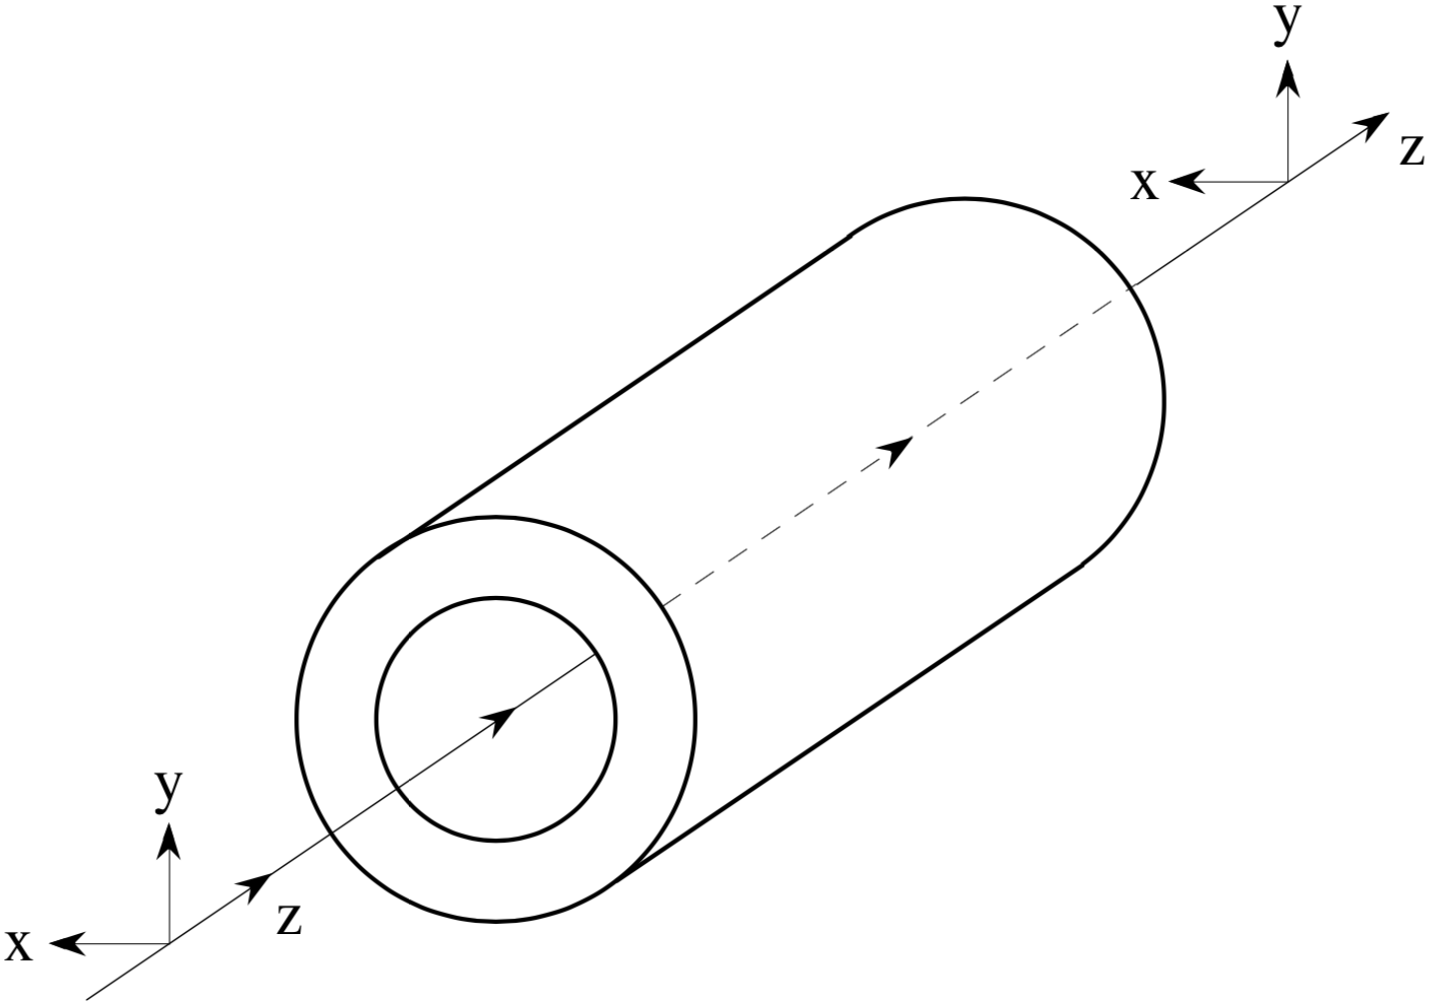
\includegraphics[scale=0.453]{SolenoidSystem}
  \caption{Coordinate system for the solenoid.}
\end{figure}

\clearpage

For simplicity, MaryLie currently provides two soft-edge ``bump" function models for the on-axis longitudinal field of the form
\[ B_z(0,0,z) = B \mbox{ bump}(z,cl,L).  \]
As described below, one corresponds to a simple air-core solenoid with a single winding, and the other models an iron-dominated solenoid.  Both have physically reasonable properties that should be adequate for at least preliminary calculations.  However, if the user wishes to make detailed calculations for a particular solenoid, he or she may wish to modify various \Mary subroutines to incorporate an improved model.

The soft-edge bump function has the properties
\[
\begin{array}{c}
\mbox{bump}(z,cl,L) \simeq 1 \mbox{ for } z \in [0,L], \\
\mbox{bump}(z,cl,L) \simeq 0 \mbox{ elsewhere},\\
\mbox{bump}(L/2 + w,cl,L) = \mbox{bump}(L/2 - w,cl,L), \\
\int_{-\infty}^{\infty}\mbox{bump}(z,cl,L) dz = L.
\end{array}   \]
Here $L$ is the length of the body of the solenoid.  In particular, from the results above one has the relation
\[  \int_{-\infty}^{\infty}B_z(0,0,z) dz = BL.  \]

Specifically, the soft-edge bump function is defined in terms of an approximating ``signum'' function sgn$(z,cl)$ by the relation
\[  \mbox{bump}(z,cl,L) = [\mbox{sgn}(z,cl) - \mbox{sgn}(z-L,cl)]/2.  \]

The approximating signum function is in turn defined by two possible relations.  In the air-core model the relation is
\[  \mbox{sgn}(z,cl) = z/[z^2+(cl)^2]^{1/2}.   \]
This model describes the case of a single-layer solenoid of length $L$, radius $cl$, and interior field $B$ (in the infinite-length limit). In this case the on-axis field falls off as $L(cl)^2/|z|^3$ for large distances, and the characteristic fall-off length is governed by $cl$. In the iron-dominated model the relation is
\[  \mbox{sgn}(z,cl) = \tanh(z/cl).   \]
In this case the on-axis field falls of exponentially as $\exp(-2|z/cl|)$ for large $|z|$, and the characteristic fall-off length is again governed by $cl$. This model does not correspond to any easily-described iron and current distribution.  However, it does have the property of exponential fall off, which is characteristic of all iron-dominated solenoids.

In both cases, the approximating signum function becomes the true signum function in the limit that the characteristic length $cl$ goes to zero,
\[ \lim_{cl \rightarrow 0} \mbox{sgn}(z,cl) = \mbox{sgn}(z).   \]
Recall that the true signum function has the definition
\[ \begin{array}{c}
\mbox{sgn}(z) = 1 \mbox{ if } z > 0,\\
\mbox{sgn}(z) = 0 \mbox{ if } z = 0,\\
\mbox{sgn}(z) = -1 \mbox{ if } z < 0.
\end{array}  \]
In this same limit the soft-edge bump function becomes the hard-edge bump function,
\[  \lim_{cl \rightarrow 0} \mbox{bump}(z,cl,L) = \mbox{bump}(z,L).  \]
The hard-edge bump function has the properties,
\[
\begin{array}{c}
\mbox{bump}(z,L) = 1 \mbox{ for }  z \in (0,L),\\
\mbox{bump}(0,L) = \mbox{bump}(L,L) = 1/2,\\
\mbox{bump}(z,L) = 0 \mbox{ elsewhere}.
\end{array}    \]

It follows that the characteristic length $cl$ (=P3) controls the rate of fall off of the fringe fields.  The fringe-field region is large if $cl$ is large, and vanishes as $cl$ goes to zero.

The quantities $B_z(0,0,z)$ and $B''_z(0,0,z)$ are written on the file IPROFILE\@.  This file is formatted into six columns as follows:
\begin{itemize}
  \item Column 1 contains $z$.
  \item Column 2 contains $B_z(0,0,z)$.
  \item Column 3 contains $B''_z(0,0,z)$.
  \item Column 4 contains the number 0.
  \item Column 5 contains the number 0.
  \item Column 6 contains the number 0.
\end{itemize}
As a result of the formatting the contents of IPROFILE can be plotted by any plot routine capable of plotting \Mary phase-space data.  See section 4.5.2.

Exhibit 6.23.1 shows the use of a solenoid along with two drifts to form
a simple imaging system as depicted schematically in figure 6.23.2.  It
also gives an example of the production of field profile plots.  In
particular, figures 6.23.3 and 6.23.4 show the field profiles $B_z(0,0,z)$ and $B''_z(0,0,z)$ for the solenoid of Exhibit 6.23.1.\index{profile} \index{field profile} \index{imaging system}

Since both drifts have the same length, the imaging system should have unit magnification, and the image should be inverted.  In addition, the image should be slightly rotated due to the spiral nature of charged particle trajectories in a longitudinal magnetic field.  Indeed, it can be shown that the rotation angle $\theta_r$ is given by the relation
\[  \theta_r = 1/2 \mbox{brho} \int_{-\infty}^{\infty} B_z(0,0,z) dz =
BL/(2 \mbox{brho}).  \]
For positive particles the rotation is counter-clockwise in the context
of figure 6.14.1.  Correspondingly, it is clockwise in the context of
figure 6.14.3.  That is, in the terminology  of section 6.14, the rotation
is equivalent to {\em arot}$(-\theta_r)$.  Caution: \ In the formula
above, $\theta_r$ is given in radians.  By contrast, the type code {\em
arot} requires an argument given in degrees.

Sometimes it is useful to artificially remove this rotation from the
transfer map.  (This rotation couples the horizontal and vertical phase
spaces, which may unduely complicate fitting or some other calculation.)
In that case, one should use negative integer values for the parameter JOB.

For further detail, see references listed in Chapter 11.

\newpage

\begin{footnotesize}
\begin{verbatim}
#comment
 Exhibit 6.23.1.
 This is a MARYLIE run illustrating use of the solenoid type code.
 A solenoid is combined with two drifts to produce an imaging system.
 The beam parameters are those for 800 MeV protons.
#beam
  4.881030646470486
 0.8526309382400936
  1.000000000000000
  1.000000000000000
#menu
 fileout  pmif
   1.00000000000000       12.0000000000000       3.00000000000000
 raysin   rt
   13.0000000000000       14.0000000000000      -1.00000000000000
  0.000000000000000E+00  0.000000000000000E+00  0.000000000000000E+00
 trace    rt
  0.000000000000000E+00   14.0000000000000       4.00000000000000
  0.000000000000000E+00   1.00000000000000      0.000000000000000E+00
 dr       drft
   22.8417247128300
 sol      sol
  0.000000000000000E+00   2.00000000000000       200.000000000000
   10.0000000000000       1.00000000000000      0.000000000000000E+00
 solpar   ps1
  0.500000000000000       1.00000000000000      0.100000000000000
   3.00000000000000       3.00000000000000      2.000000000000000E+00
 end      end
#lines
 lens
     1*solpar      1*sol
 image
     1*dr          1*lens        1*dr
#lumps
#loops
#labor
    1*fileout
    1*image
    1*raysin
    1*trace
    1*end

 zi=  0.0000000000000000E+00 zf=   2.000000000000000
 ns=         200
 di=  0.5000000000000000     length=   1.000000000000000
 cl=  0.1000000000000000     B=   3.000000000000000
 job=          2
\end{verbatim}
\end{footnotesize}

\newpage

\begin{figure}[p]
  \centering
  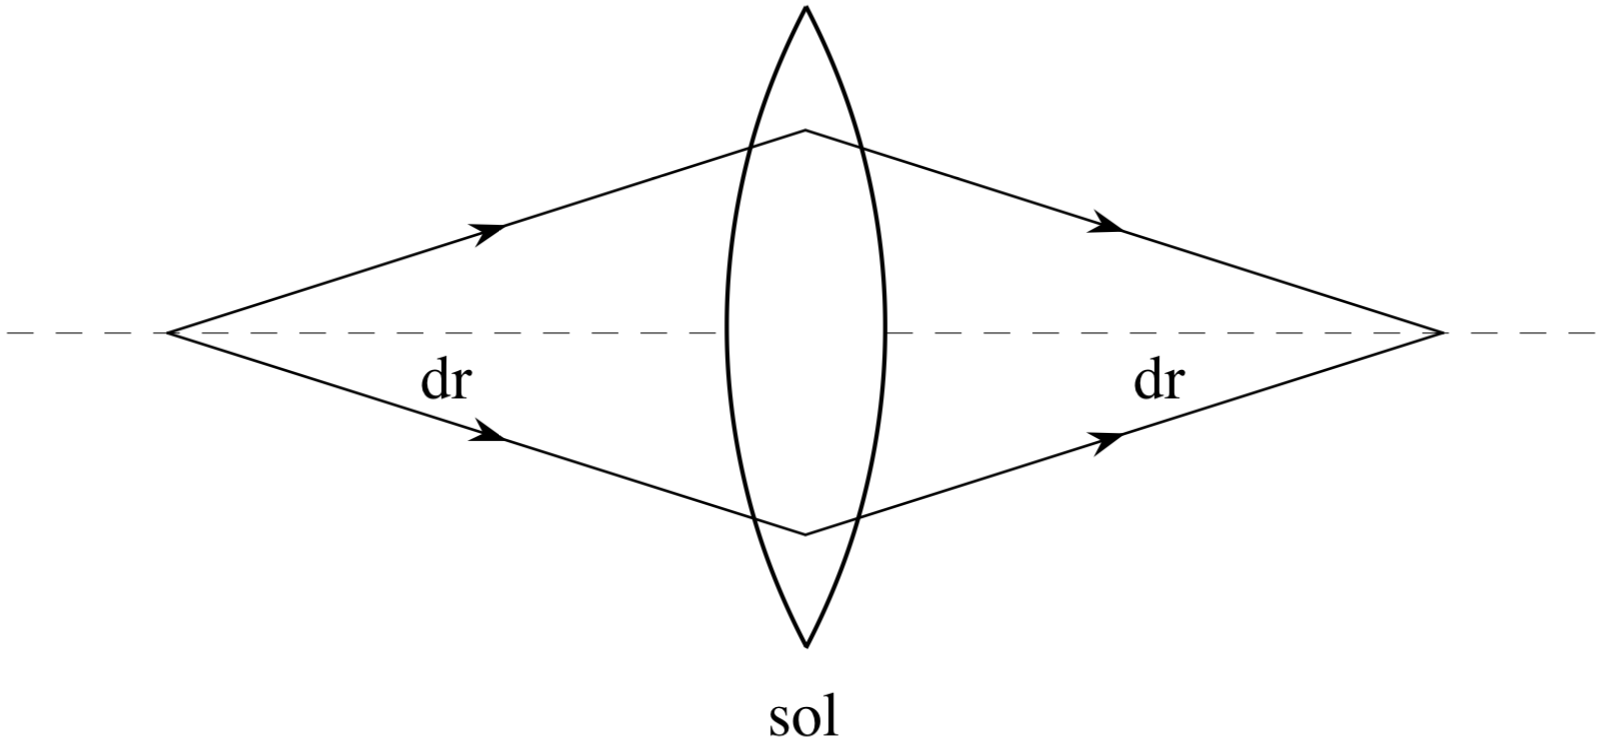
\includegraphics[scale=0.453]{ImagingSystem}
  \caption{Schematic of the imaging system of Exhibit 6.23.1.}
\end{figure}

\clearpage

\begin{figure}[p]
  \centering
  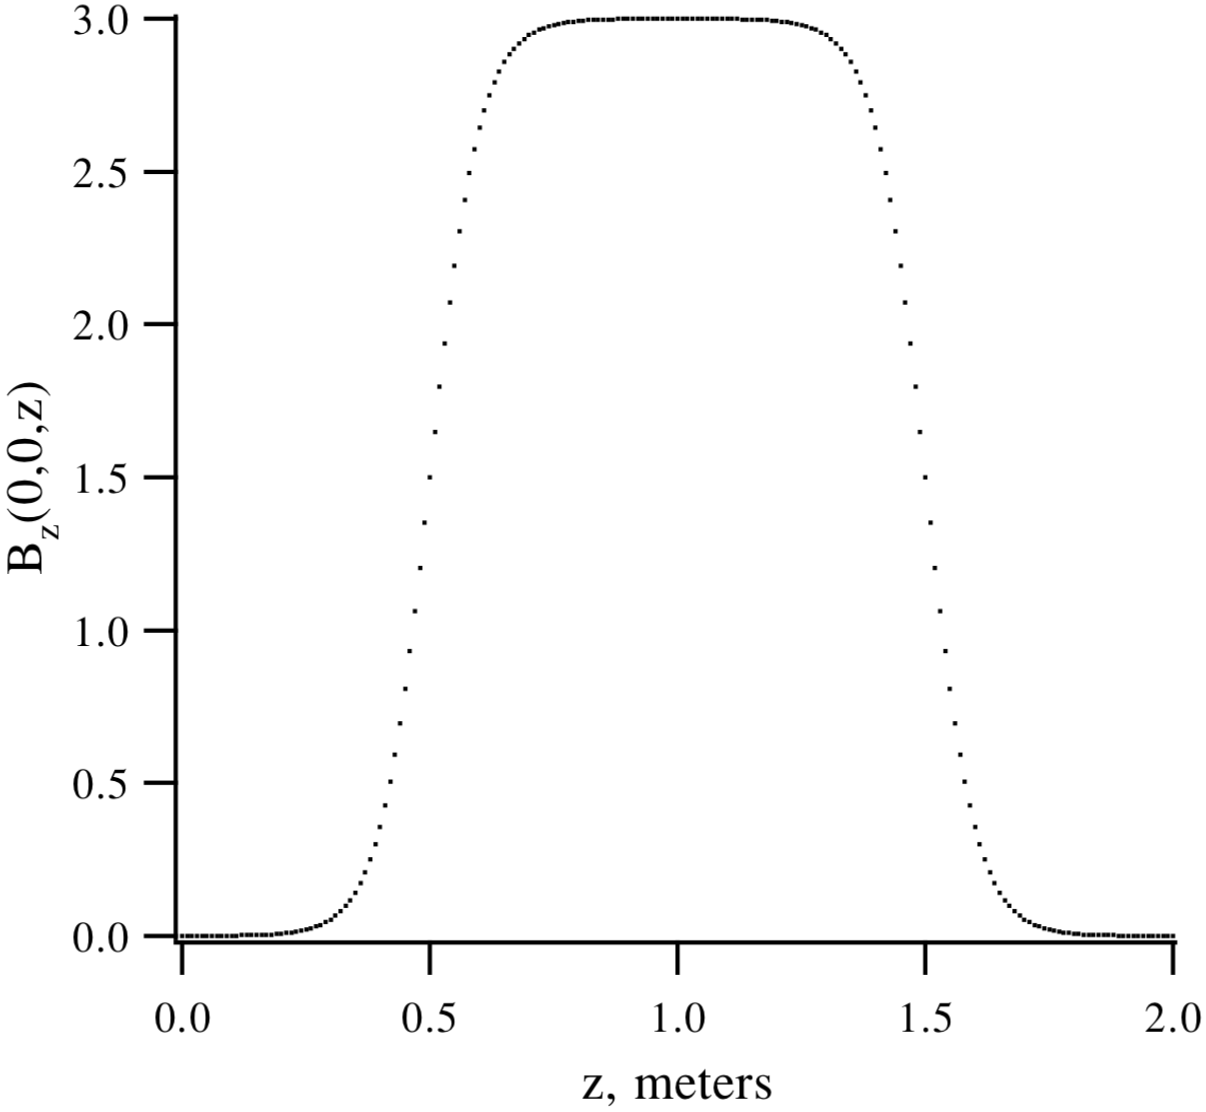
\includegraphics[scale=0.453]{sol1}
  \caption{Profile of $B_z(0,0,z)$, (Tesla), for the solenoid of Exhibit 6.23.1.  Parameter values are DI=.5, $L=1$, $cl=.1$, and $B=3$.}
\end{figure}

\begin{figure}[p]
  \centering
  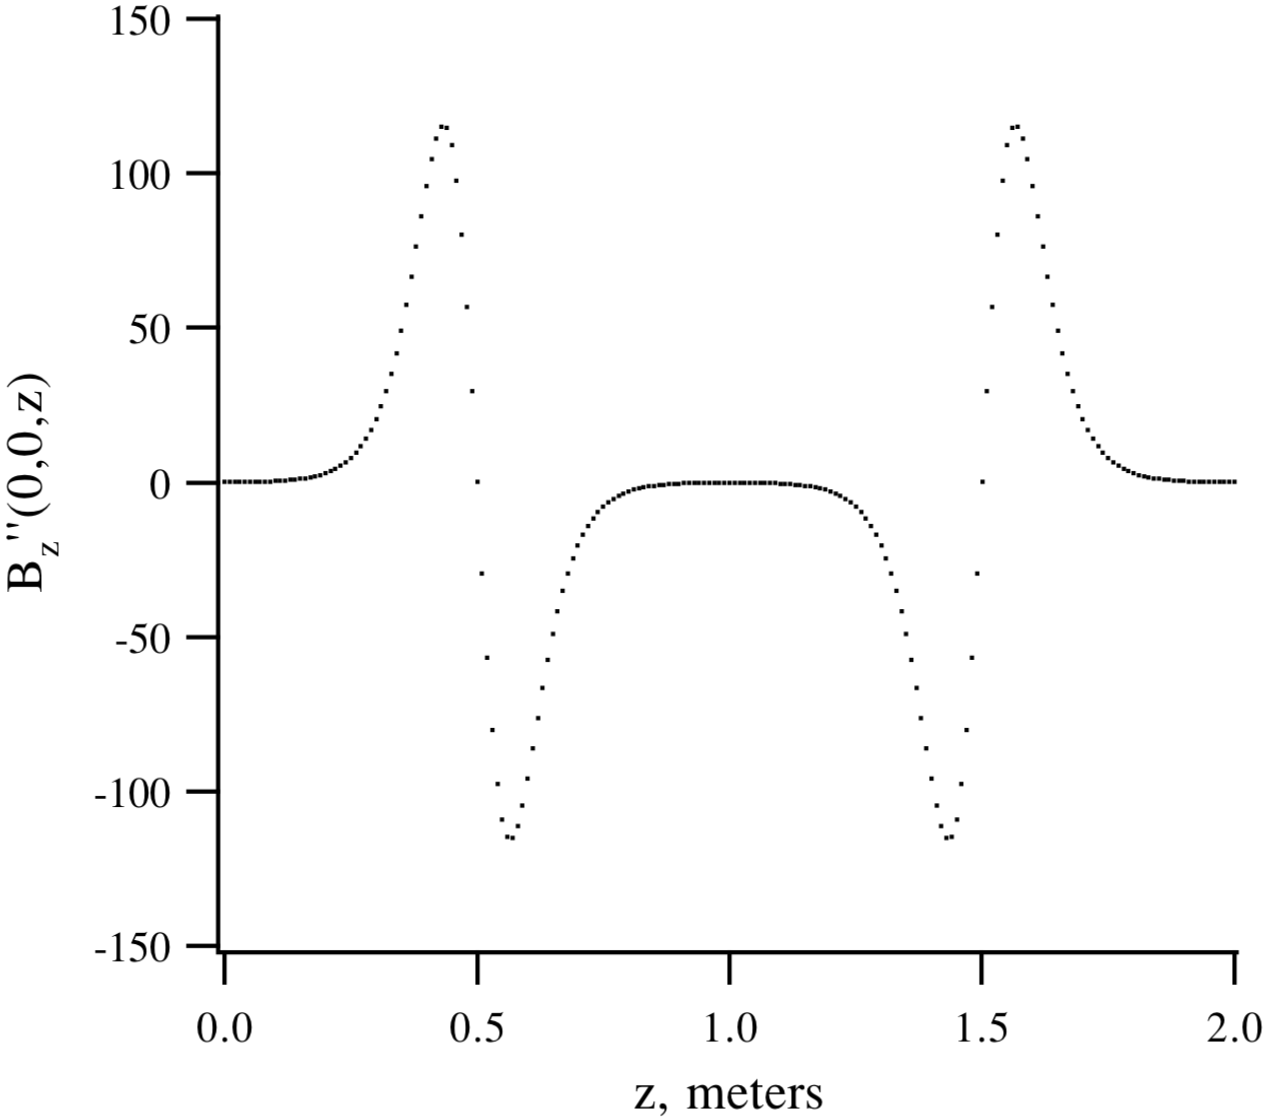
\includegraphics[scale=0.453]{sol2}
  \caption{Profile of $B''_z(0,0,z)$, (Tesla/m$^2$), for the solenoid of Exhibit 6.23.1.  Parameter values are DI=.5, $L=1$, $cl=.1$, and $B=3$.}
\end{figure}

\clearpage

How well does this system work in practice?  Suppose the word MARYLIE, as
shown in figure 2.3.4, is used as an object.  Figure 6.23.5 shows the image produced.  Evidently the image is inverted and rotated as expected.  It can also be shown that there is unit magnification near the origin.  However, it is evident that there are very severe aberrations  away from the origin!  Indeed, these aberrations are so severe that third-order results alone may be insufficient to describe the outer parts of the image.\index{aberrations}

It can be shown that the third and higher order aberrations of a solenoid
become infinite in the hard-edge limit ($cl$ goes to zero).  Thus, the hard-edge limit is unphysical for a solenoid.  Correspondingly, third-order solenoid aberrations can be reduced by making the fringe-field region large.  It also helps to make the solenoid weak since aberrations are proportional to $B$.  If this is done, the solenoid must also be made long (to compensate for the small $B$) in order to maintain the desired paraxial properties.\index{fringe field}

\begin{figure}[hp]
  \centering
  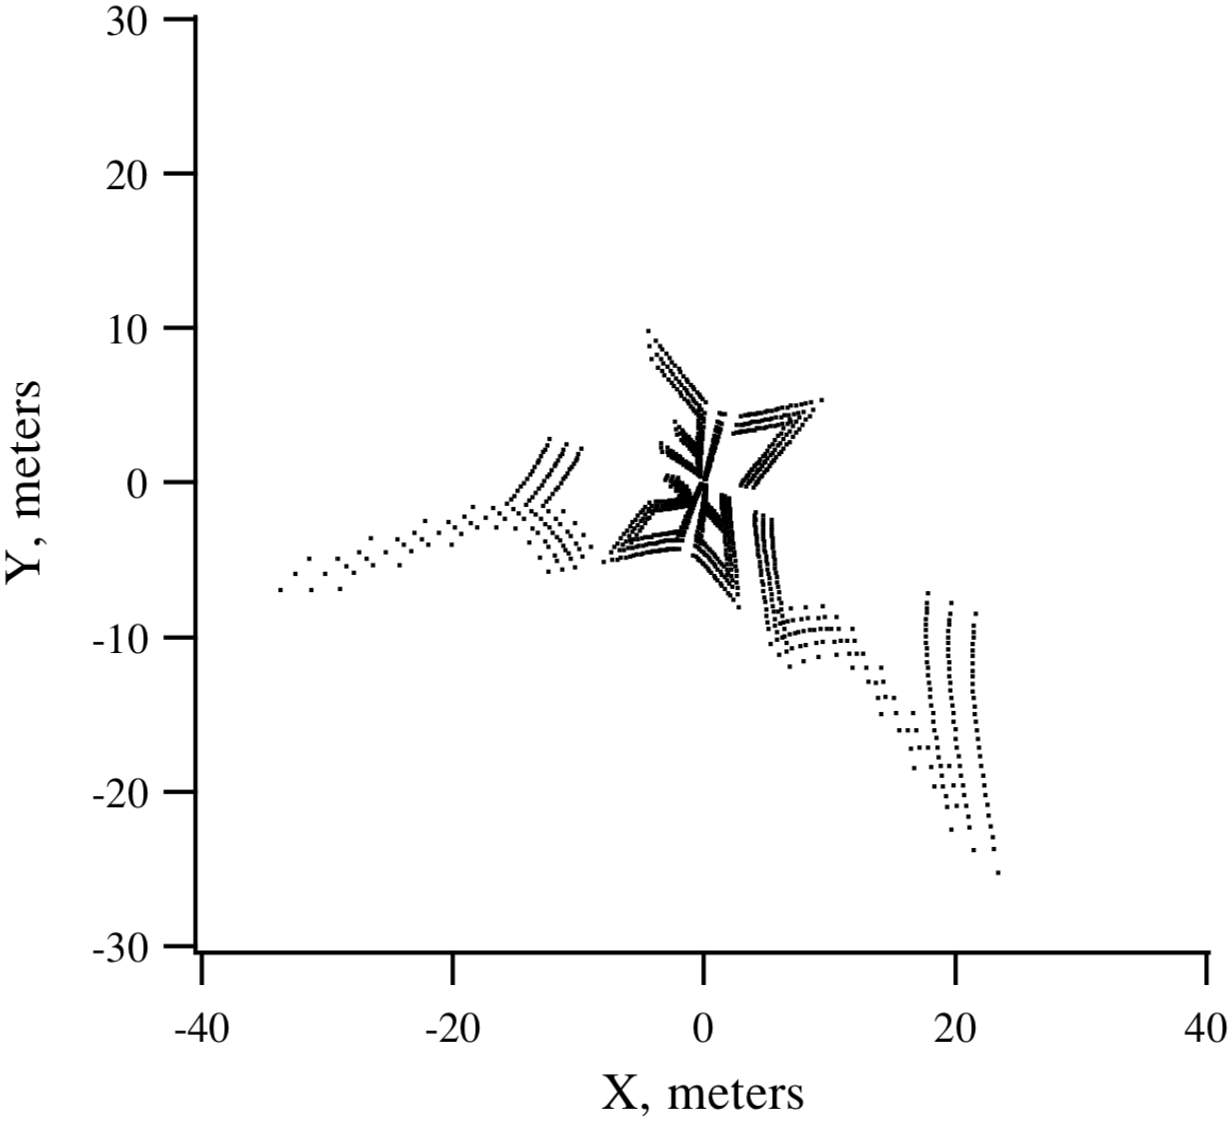
\includegraphics[scale=0.453]{solimage}
  \caption{Image of the word MARYLIE produced by the simple imaging system of Exhibit 6.23.1.}
\end{figure}

\clearpage



\section{Combined Function Magnetic Quadrupole}
\begin{quotation}
\noindent Type Code:  cfqd\index{combined function quadrupole} \index{multipole} \index{quadrupole}
\vspace{5mm}

\noindent Required Parameters:
\begin{enumerate}
      \item  Length of quadrupole (m).

      \item  IPSET

             = 0 to set all multipole coefficients to zero.

             = J (with J an integer from 1 to 9) to take multipole
               coefficient values from \hspace*{1em}the parameter set associated with
               the type code {\em psj}.  (See section 7.25.)  \hspace*{1em}In this case
               the parameters P1\ldots P6 from the parameter set associated
               \hspace*{1em}with {\em psj } are used as follows:

           \hspace*{2em}  P1 = BQD (Tesla/m) \hspace{1em} (normal)

           \hspace*{2em}  P2 = AQD (Tesla/m) \hspace{1em} (skew)

           \hspace*{2em}  P3 = BSEX (Tesla/$\mbox{m}^2$) \hspace{1em} (normal)

           \hspace*{2em}  P4 = ASEX (Tesla/$\mbox{m}^2$) \hspace{1em} (skew)

           \hspace*{2em}  P5 = BOCT (Tesla/$\mbox{m}^3$) \hspace{1em} (normal)

           \hspace*{2em}  P6 = AOCT (Tesla/$\mbox{m}^3$) \hspace{1em} (skew)

      \item  LFRN

             = 0 for no fringe field on leading edge (entry) of quadrupole.

             = 1 for hard-edge fringe field on leading edge of quadrupole.

      \item  TFRN

             = 0 for no fringe field on trailing edge (exit) of quadrupole.

             = 1 for hard-edge fringe field on trailing edge of quadrupole.
\end{enumerate}

\vspace{5mm}
\noindent     Example:
\begin{verbatim}
          allcfqd   cfqd
          .5 , 1 , 1 , 1
\end{verbatim}
\end{quotation}
The above specifies a combined function magnetic quadrupole with user
given name {\em allcfqd}.  It has a length of .5 meters and has hard-edge
leading and trailing fringe fields.  Multipole coefficient values are
taken from parameter set 1.  Suppose the parameter values in parameter
set 1 have been set by previously invoking in \#labor the following command:
\begin{quotation}
\begin{verbatim}
          allpar      ps1
          2.5 , .2 , .3 , .4 , .5 , .6
\end{verbatim}
\end{quotation}
Then the normal quad strength is 2.5 Tesla/m, and, in the absence of
other multipoles, the quadrupole would be horizontally focusing.
However, there are also other multipoles:  the skew quad strength is .2
Tesla/m, the normal sextupole strength is .3 Tesla/$\mbox{m}^2$,
the skew sextupole strength is .4 Tesla/$\mbox{m}^2$, the normal
octupole strength is .5 Tesla/$\mbox{m}^3$, and the skew octupole
strength is .6 Tesla/$\mbox{m}^3$.

\vspace{5mm}
      Description:
\vspace{2mm}

      A combined function quadrupole is a quadrupole with added sextupole
and octupole components.  Thus, pure quadrupoles, pure sextupoles, and pure
octupoles are special cases of the combined function quadrupole.  As
illustrated in Exhibit 6.24.1, the combined function quadrupole is,
in turn, a special limiting case of the combined function bend.

\clearpage
\begin{footnotesize}
\begin{verbatim}
#comment
 Exhibit 6.24.1.
 This is a MARYLIE run illustrating the sign conventions for
 combined function magnetic quadrupoles.  A combined function
 magnetic quadrupole is a quadrupole with added sextupole and
 octupole components.  Thus, pure quadrupoles, pure sextupoles,
 and pure octupoles are special cases of the combined function
 quadrupole.  In this run a comparison is made with the combined
 function bend in the limit of no dipole field.  Note that to
 obtain a finite length element without dipole content using
 the cfbd element, it is necessary to make both the dipole field
 small and the bend angle small in such a way that the design orbit
 path length as given in figure 6.2a takes on the desired value.
 For simplicity of calculation the value of brho has been set
 equal to 10/pi.  Thus, the path length is given by the relation

  path length = 10/180 * theta (in degrees) /B.

 In particular, if

      theta = 9.e-9 and B = 1.e-9,
 then

       path length = .5 meters.

#beam
  3.183098861830000
 0.8526309382400936
  1.000000000000000
  1.000000000000000
#menu
 fileout  pmif
   1.00000000000000       12.0000000000000       3.00000000000000
 setzero  zer
  0.000000000000000E+00  1.000000000000000E-08  0.000000000000000E+00
 mapout   ptm
   3.00000000000000       3.00000000000000      0.000000000000000E+00
  0.000000000000000E+00   1.00000000000000
 wcfbd    cfbd
  9.000000000000000E-09  1.000000000000000E-09   1.00000000000000
   1.00000000000000       1.00000000000000       1.00000000000000
 fcfbdpar ps1
   5.00000000000000       2.50000000000000       20.0000000000000
   30.0000000000000       40.0000000000000       50.0000000000000
 dcfbdpar ps1
  -5.00000000000000       2.50000000000000       20.0000000000000
   30.0000000000000       40.0000000000000       50.0000000000000
 cfqd    cfqd
  0.500000000000000       1.00000000000000       1.00000000000000
   1.00000000000000
 clear    iden
 inv      inv
 end      end
#lines
 tfcfbd
     1*fcfbdpar    1*wcfbd
 tdcfbd
     1*dcfbdpar    1*wcfbd
 tfcfqd
     1*fcfbdpar     1*cfqd
 tdcfqd
     1*dcfbdpar     1*cfqd
 test
     1*clear       1*tfcfbd      1*inv         1*tfcfqd      1*mapout   &
     1*clear       1*tdcfbd      1*inv         1*tdcfqd      1*mapout
#lumps
#loops
#labor
    1*fileout
    1*setzero
    1*test
    1*end
\end{verbatim}
\end{footnotesize}
Results of test
\begin{footnotesize}
\begin{verbatim}
matrix for map is :

  1.00000E+00  1.24184E-12  1.27068E-16 -3.98986E-17  0.00000E+00  4.51475E-11
 -1.95069E-12  1.00000E+00  9.76028E-13 -9.71445E-17  0.00000E+00  1.74682E-10
 -9.36751E-17  1.64799E-17  1.00000E+00  1.24192E-12  0.00000E+00  7.63386E-13
  9.74838E-13  6.24500E-17  1.95086E-12  1.00000E+00  0.00000E+00  6.10779E-12
 -1.74682E-10  4.51475E-11 -6.10779E-12  7.63386E-13  1.00000E+00  5.10553E-13
  0.00000E+00  0.00000E+00  0.00000E+00  0.00000E+00  0.00000E+00  1.00000E+00

 nonzero elements in generating polynomial are :


 matrix for map is :

  1.00000E+00  1.24191E-12 -9.58435E-17  1.73472E-17  0.00000E+00  4.82011E-11
  1.95084E-12  1.00000E+00  9.74811E-13  6.76542E-17  0.00000E+00  1.99113E-10
  1.17961E-16 -3.90313E-17  1.00000E+00  1.24183E-12  0.00000E+00  7.63386E-13
  9.76004E-13 -8.50015E-17 -1.95068E-12  1.00000E+00  0.00000E+00  6.10779E-12
 -1.99113E-10  4.82011E-11 -6.10779E-12  7.63386E-13  1.00000E+00  5.10553E-13
  0.00000E+00  0.00000E+00  0.00000E+00  0.00000E+00  0.00000E+00  1.00000E+00

nonzero elements in generating polynomial are :

\end{verbatim}
\end{footnotesize}

\newpage




\section{Marker}
\begin{quotation}
\noindent Type Code:  mark\index{marker}
\vspace{5mm}

\noindent Required Parameters:  None

\vspace{5mm}
\noindent Example:
\begin{verbatim}
          spot1      mark
\end{verbatim}
\end{quotation}
This specifies a marker with user given name {\em spot1}.

\vspace{5mm}
     Description:
\vspace{2mm}

     These elements have no direct effect in a \Mary run.  They simply
	 afford the user the opportunity to give names to various locations in a lattice or beam line.

\newpage



\section{Data Point}\index{data point}
\begin{quotation}
\noindent Type Code:  dp
\vspace{5mm}

\noindent Required Parameters:  None

\vspace{5mm}
\noindent Example:
\begin{verbatim}
          point1      dp
\end{verbatim}
\end{quotation}

\vspace{5mm}
     Description:
\vspace{2mm}

     These elements are recognized by the {\em geom} type code and are
	 used for producing graphics.  See sections 8.38, 10.9, and 10.11
	 through 10.14.

\newpage


\section{Rare Earth Cobalt (REC) Quadrupole Multiplet}
\begin{quotation}
\noindent     Type Code:  recm\index{REC quadrupole} \index{quadrupole} \index{multipole} \index{multiplet}
\vspace{5mm}

\noindent     Required Parameters:
\begin{enumerate}
       \item  zi (initial longitudinal coordinate in meters).
       \item  zf (final longitudinal coordinate in meters).
       \item  NS (number of integration steps).
       \item  IPROFILE

              = 0 to not write out field profile.

              = IFILE to write profile on file IFILE.

              Note:  If IFILE$<0$, the effect is the same as when IFILE$>0$ except that
              only the profile is computed and the numerical integration required to
              compute the map specified by {\em recm} is bypassed.  Instead, the identity
              map is returned.  This feature makes it possible to compute profiles, if
              that is all that is desired, without spending time on unnecessary numerical
              integration.
       \item  MULTIPOLES

              = 0 to set all higher multipole coefficients to zero.

              = index (an integer from 1 to 9) of parameter set containing multipole
              \hspace*{1.2em}strength information for the region of integration zi,zf.

              \item  NPAT (index of parameter set containing quadrupole pattern
              information, an integer from 1 to 9).
\end{enumerate}
\end{quotation}
This element also requires additional parameters whose values are specified
by the parameter sets with indices MULTIPOLES, NPAT, and IPS, IPS$+$1,\ldots, (IPS$+$NTSEC$-$1).
See section 7.25.  The contents of the parameter set with index MULTIPOLES are as follows:
\begin{enumerate}
  \item  BSEX (Tesla/$\mbox{m}^2$). \hspace{1em} (normal)
  \item  ASEX (Tesla/$\mbox{m}^2$). \hspace{1em} (skew)
  \item  BOCT (Tesla/$\mbox{m}^3$). \hspace{1em} (normal)
  \item  AOCT (Tesla/$\mbox{m}^3$). \hspace{1em} (skew)
  \item  0 (not used, but must be present).
  \item  0 (not used, but must be present).
\end{enumerate}
The contents of the parameter set with index NPAT control and describe the pattern of quadrupoles as follows:
\begin{enumerate}
  \item  DI (length of initial drift space in front of pattern, starting from $z=0$, in meters).
  \item  NTSEC (number of types of quadrupole sections to be described by additional parameter sets).  Note:  This number must currently be limited to be less than or equal to 9.
  \item  IPS (index of first parameter set describing the first section of quadrupoles).  \linebreak Subsequent parameter sets used to describe additional sections have indices \linebreak IPS$+$1\ldots (IPS$+$NTSEC$-$1).
  \item  MAXSEC (maximum number of sections to be used in quadrupole pattern or repeated quadrupole pattern).
  \item  NCYC (number of cycles through pattern, except that the sequence of sections terminates when the number of sections employed reaches MAXSEC).
  \item  ISEND

         =0 to not write out pattern.

         =1 to write pattern at the terminal.

         =2 to write pattern on file 12.

         =3 to write pattern at the terminal and on file 12.
\end{enumerate}
Finally, the contents of the NTSEC parameter sets with indices \linebreak IPS \ldots (IPS$+$NTSEC$-$1) define the type and number of quadrupoles in each section as follows:
\begin{enumerate}
  \item  Length $L$ of quadrupole (m).
  \item  Strength $Q$ of quadrupole, if it were infinitely long (Tesla/m).
  \item  Inner radius (m).
  \item  Outer radius (m).
  \item  Length of trailing drift space after quadrupole (m).  Note that
the length assigned to the trailing drift after the {\em last} quadrupole in the whole pattern or repeated pattern is ignored.  The integration always stops at zf.
  \item  NQUAD [number of (identical) quadrupoles that appear in the section].
\end{enumerate}

\vspace{5mm}
\begin{quotation}
\noindent     Example:

    See Exhibits 6.27.1 through 6.27.3 and figures 6.27.1 through 6.27.3.
\end{quotation}

\vspace{5mm}
     Description:
\vspace{2mm}

     The type code {\em recm} has great flexibility at the cost of some
complexity.  It causes the production of the transfer map for a part or
all of a collection of REC quadrupoles that will be referred to as
``whole''.  This is done by numerical integration over the interval from
zi to zf in NS steps using a special purpose built-in GENMAP routine.
(See section 1.4.1).  Superimposed on the interval zi,zf is a (piece-wise
constant) multipole (sextupole plus octupole) magnetic field.\index{GENMAP}

     The accuracy of the numerical integration procedure depends on the number NS of integration steps employed and the spatial rate of variation of the magnetic field.  The more rapidly the field varies, the more steps are required.  Therefore, the user should try several values for NS to be sure that sufficient accuracy has been achieved.  Increasing NS improves the accuracy, but also increases the computation time.

     The contents of ``whole'' is equivalent to the following sequence of \linebreak
     \Mary lines:

\begin{tabbing}
\tt \#lines\\
\tt whole\\
 \ \ \=\tt drin\ \ \= \  \ \=\tt rpattern\\
        \>\> ({\em drin } is an initial drift with length DI;  {\em rpattern } refers to\\
        \>\> ``repeated pattern'' as defined in the next line)\\
\tt rpattern\\
\>\tt  NCYC*pattern\\
\tt pattern\\
\>\tt  sect1           \>\>\tt sect2 $\cdots$ sectNTSEC\\
\tt sect1\\
\>\tt   NQUAD1*pair1\\
\tt sect2\\
\>\tt   NQUAD2*pair2\\
\>\>\>$\vdots$ \\
\tt sectNTSEC\\
\>\tt NQUADNTSEC*pairNTSEC\\
\tt pair1\\
\>\tt quad1\>\>\tt tdr1\\
\tt pair2\\
\>\tt quad2\>\>\tt tdr2\\
\>\>\>$\vdots$\\
\tt pairNTSEC\\
\>\tt quadNTSEC\ \ \ \ tdrNTSEC\\
\>\>(here {\em quadj} and {\em tdrj} refer to the quadrupole and trailing drift\\
\>\>pair in the $\mbox{j}^{\mbox{\scriptsize th}}$ section)
\end{tabbing}
However, it is to be understood that all of {\em rpattern} is not used if NCYC*NTSEC exceeds MAXSEC.  In this case, only the first MAXSEC sections in {\em rpattern } are used.  Also, it should be understood that the magnetic field at any integration point is the superimposed multipole field plus the sum of all REC quadrupole fields in the pattern, repeated pattern, or MAXSEC sections (whichever is applicable).  Thus, the type code {\em recm} includes the effect of overlapping fringe fields.\index{fringe field}  Finally, the ability to superimpose multipole fields makes it possible, if desired, to add (piece-wise constant) sextupole and octupole content to each REC quadrupole.

It can be shown that the vector potential for a quadrupole configuration is (through fourth order) of the form
\begin{eqnarray*}
A_x &=&  \frac{g'(z)}{4}(x^3-xy^2),\\
A_y &=&  -\frac{g'(z)}{4}(y^3-x^2 y),\\
A_z &=&  -\frac{g(z)}{2} (x^2-y^2) + \frac{g''(z)}{12} (x^4-y^4).
\end{eqnarray*}
Here $g(z)$ is the on-axis field gradient, and the quantities $g'(z)$ and $g''(z)$ are derivatives of $g$ with respect to $z$.

For a single REC quadrupole of length $L$ and strength $Q$ with entrance
face at $z=0$ (and exit face at $z=L$), it can be shown that $g(z)$ has the following properties:
\begin{eqnarray*}
g(z)  \simeq  Q \ {\rm for}  \ z\in [0,L],\\
g(z)  \simeq  0 \ {\rm elsewhere},\\
g(\frac{L}{2}+w)  =  g(\frac{L}{2}-w),\\
\int_{-\infty}^{\infty} g(z)dz  =  QL.
\end{eqnarray*}
For a description of REC quadrupoles and the computation of $g(z)$, see
the reference to the work of Halbach in Chapter 11.

The quantities $g$, $g'$, $g''$ as a function of $z$ are written on file IPROFILE.  This file is formatted into six columns as follows:
\begin{enumerate}
   \item  Column 1 contains $z.$
   \item  Column 2 contains $g(z).$
   \item  Column 3 contains $g'(z).$
   \item  Column 4 contains $g''(z).$
   \item  Column 5 contains the number 0.
   \item  Column 6 contains the number 0.
\end{enumerate}
As a result of this formatting the contents of IPROFILE can be plotted by any plot routine capable of plotting \Mary phase-space data.  See section 4.5.2.

Figures 6.27.1 through 6.27.3 show the field profiles $g$, $g'$, and
$g''$ for the soft-edge REC quadrupole singlet of Exhibit 6.27.1.  Figure
6.27.4 shows the gradient $g$ for the REC quadrupole singlet of Exhibit 6.27.1 when the inner radius is very small.  In this case the profile is essentially that of a hard-edge quadrupole.\index{profile} \index{field profile} \index{singlet}

\newpage
\begin{figure}[h]
  \centering
  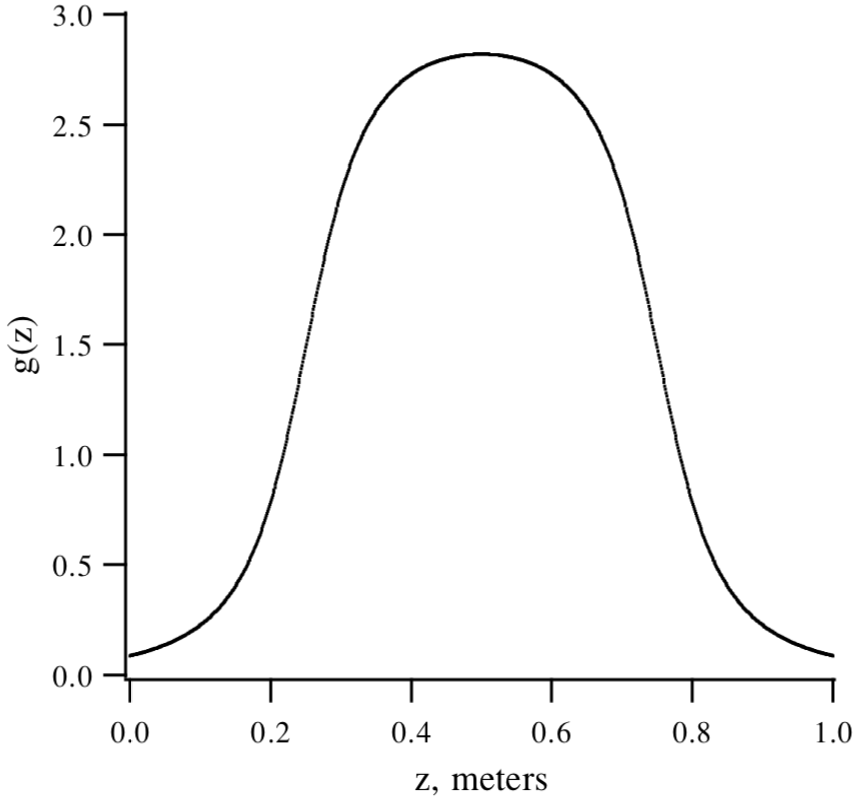
\includegraphics[height=2.55in]{recsinglet1}
  \caption{Profile of $g(z)$, (Tesla/m), for the soft-edge REC quadrupole singlet of Exhibit 6.27.1.}
\end{figure}

\begin{figure}[h]
  \centering
  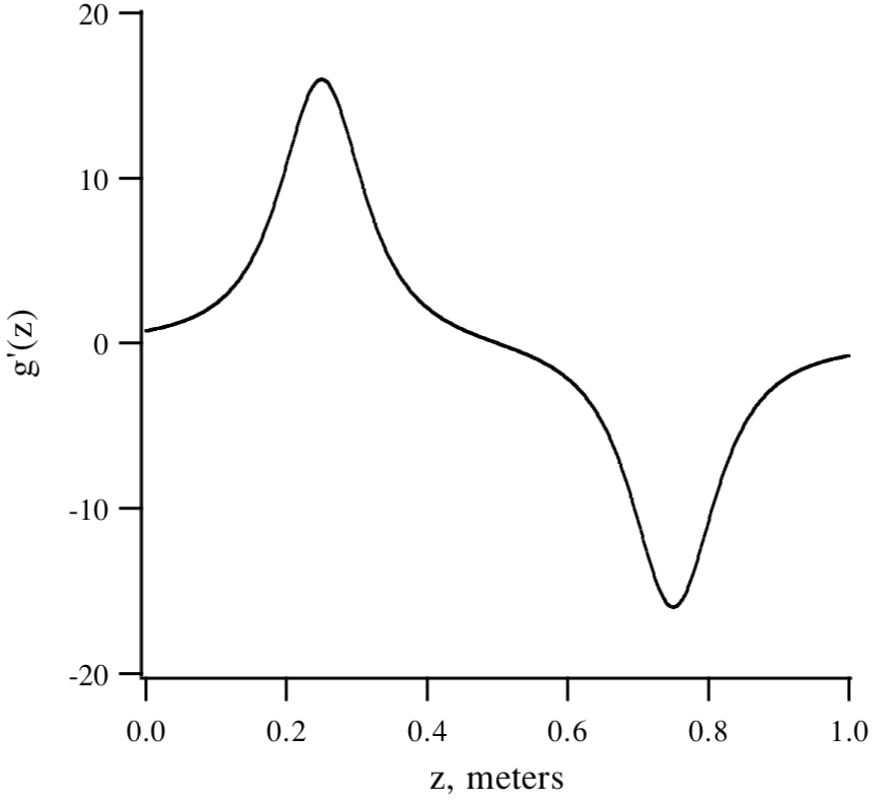
\includegraphics[height=2.55in]{recsinglet2}
  \caption{Profile of $g'(z)$, (Tesla/$\mbox{m}^2$), for the soft-edge REC quadrupole single of Exhibit 6.27.1.}
\end{figure}

\newpage
\begin{figure}[h]
  \centering
  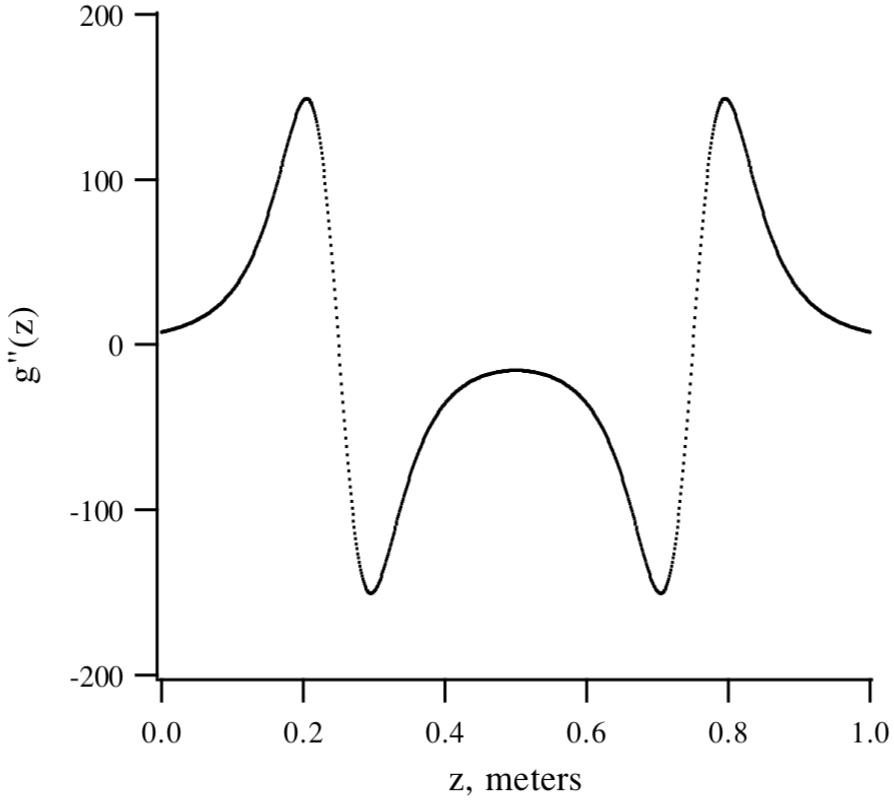
\includegraphics[height=2.55in]{recsinglet3}
  \caption{Profile of $g''(z)$, (Tesla/$\mbox{m}^3$), for the soft-edge REC quadrupole singlet of Exhibit 6.27.1.}
\end{figure}

\begin{figure}[h]
  \centering
  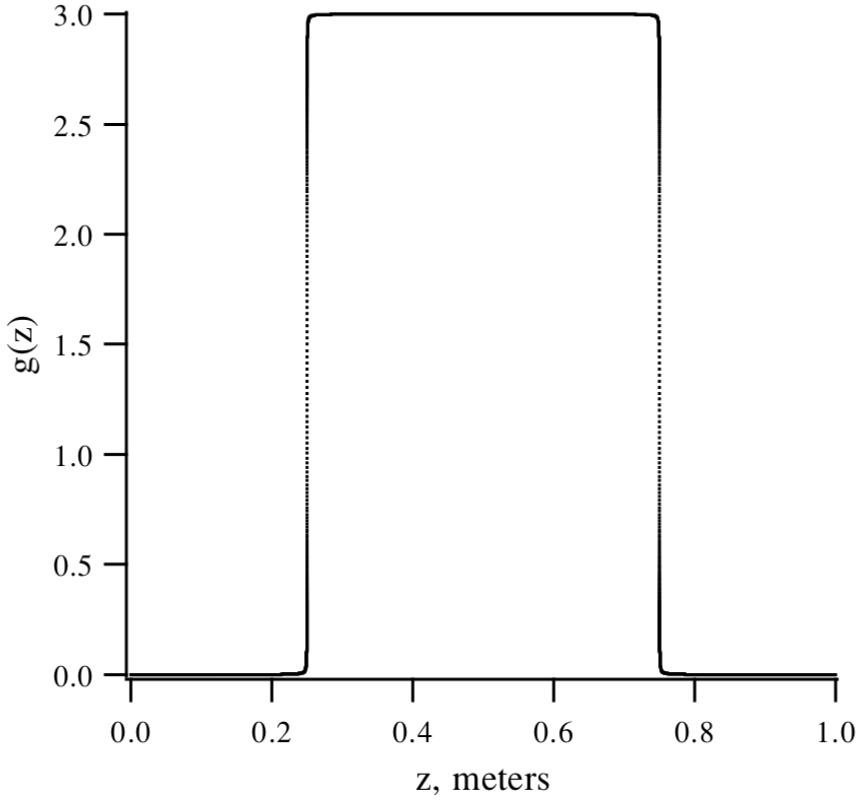
\includegraphics[height=2.55in]{recsmallsinglet}
  \caption{Profile of $g(z)$, (Tesla/m), for the very small bore REC quadrupole singlet of Exhibit 6.27.1.  In this case, the profile is essentially that of a hard-edge quadrupole.}
\end{figure}

\newpage
Figures 6.27.5 and 6.27.6 and Exhibits 6.27.2 and 6.27.3 illustrate the use of the type code {\em recm} to produce REC quadrupole doublets and triplets.  Should the user wish to treat more complicated REC quadrupole arrays, she or he is encouraged to check that the proper gradient profile is indeed being produced.\index{doublet} \index{triplet}

\newpage
\begin{figure}[h]
  \centering
  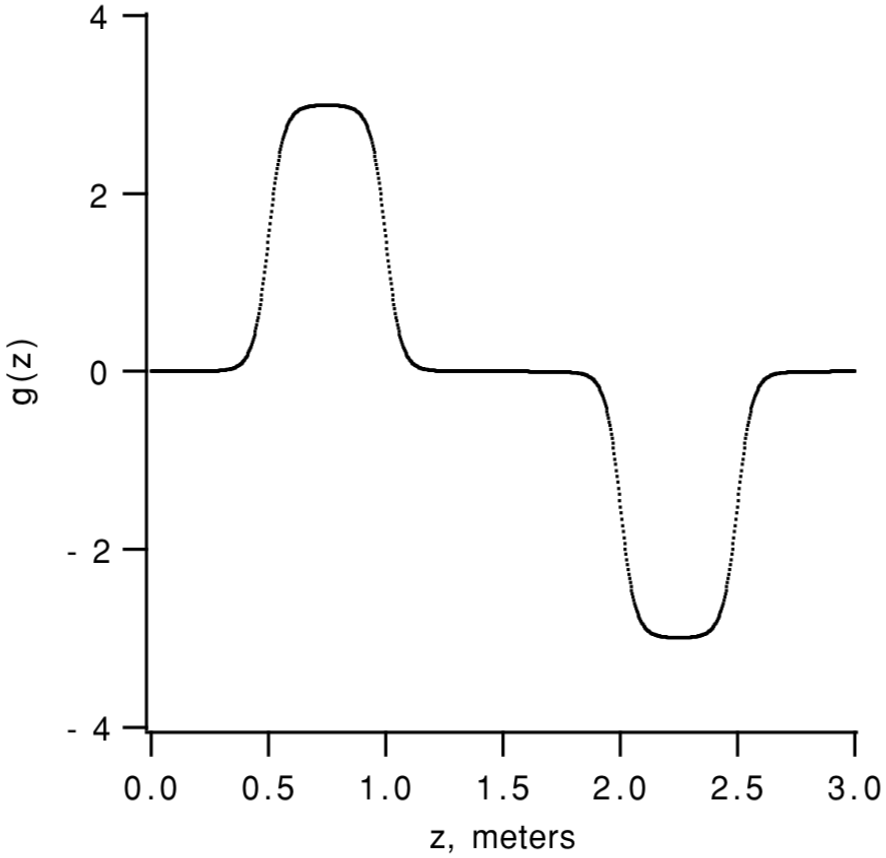
\includegraphics[height=2.71in]{recdoublet}
  \caption{Profile of $g(z)$, (Tesla/m), for the soft-edge REC quadrupole doublet of Exhibit 6.27.2.}
\end{figure}

\begin{figure}[h]
  \centering
  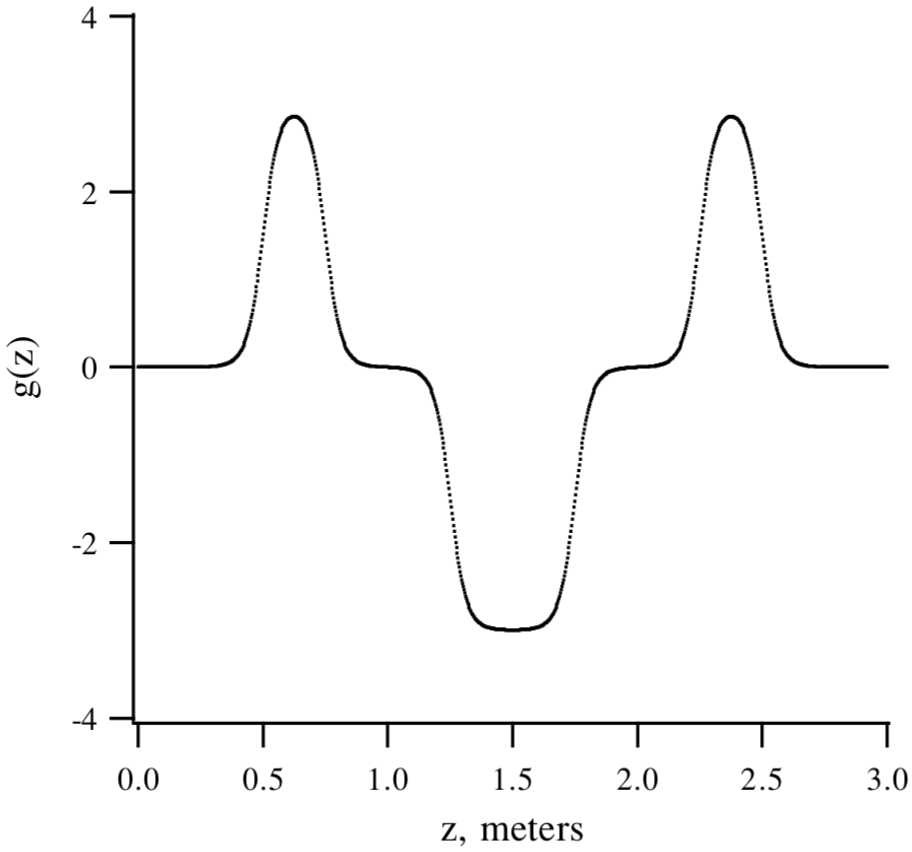
\includegraphics[height=2.71in]{rectriplet}
  \caption{Profile of $g(z)$, (Tesla/m), for the soft-edge REC quadrupole triplet of Exhibit 6.27.3.}
\end{figure}

\newpage
\begin{footnotesize}
\begin{verbatim}
 #comment
  Exhibit 6.27.1.
  This is a MARYLIE input file to test a REC quadrupole singlet.
  First the map is computed for a typical REC quadrupole that has
  soft edges.  Next the inner radius is made very small so that
  the edges in effect become hard, and comparison is made with the
  the map for the standard MARYLIE hard-edge quadrupole to show
  that in the hard-edge limit the two maps agree.  Comparison is
  also made with a standard MARYLIE quadrupole with hard-edge
  fringe fields turned off to show that these effects are important.
  Note that the limiting process is quite delicate.  The integration
  region has to be broken up into separate pieces, and a large
  number of steps is required in the fringe field regions where
  the field is changing very rapidly.
  The beam parameters are those for 800 MeV protons.
 #beam
   4.881030646470486
  0.8526309382400936
   1.000000000000000
   1.000000000000000
 #menu
  setzero  zer
   0.000000000000000E+00  1.000000000000000E-14  0.000000000000000E+00
  fileout  pmif
    1.00000000000000       12.0000000000000       3.00000000000000
  mapout   ptm
    3.00000000000000       3.00000000000000      0.000000000000000E+00
   0.000000000000000E+00   1.00000000000000
  srecm    recm
   0.000000000000000E+00   1.00000000000000       1000.00000000000
    20.0000000000000       1.00000000000000       2.00000000000000
  ldrecm   recm
   0.000000000000000E+00  0.240000000000000       1000.00000000000
    22.0000000000000       1.00000000000000       2.00000000000000
  lffrecm  recm
   0.240000000000000      0.260000000000000       10000.0000000000
    22.0000000000000       1.00000000000000       2.00000000000000
  bdrecm   recm
   0.260000000000000      0.740000000000000       1000.00000000000
    22.0000000000000       1.00000000000000       2.00000000000000
  tffrecm  recm
   0.740000000000000      0.760000000000000       10000.0000000000
    22.0000000000000       1.00000000000000       2.00000000000000
  tdrecm   recm
   0.760000000000000       1.00000000000000       1000.00000000000
    22.0000000000000       1.00000000000000       2.00000000000000
  mpoles   ps1
   0.000000000000000E+00  0.000000000000000E+00  0.000000000000000E+00
   0.000000000000000E+00  0.000000000000000E+00  0.000000000000000E+00
  npatps   ps2
   0.250000000000000       1.00000000000000       3.00000000000000
    1.00000000000000       1.00000000000000       3.00000000000000
  npatpsq  ps2
   0.250000000000000       1.00000000000000       3.00000000000000
    1.00000000000000       1.00000000000000      0.000000000000000E+00
  stype1   ps3
   0.500000000000000       3.00000000000000      0.100000000000000
   0.700000000000000      0.250000000000000       1.00000000000000
  htype1   ps3
   0.500000000000000       3.00000000000000      1.000000000000000E-04
   0.700000000000000      0.250000000000000       1.00000000000000
  dr       drft
   0.250000000000000
  hfqwff   quad
   0.500000000000000       3.00000000000000       1.00000000000000
    1.00000000000000
  hfqwoff  quad
   0.500000000000000       3.00000000000000      0.000000000000000E+00
   0.000000000000000E+00
  clear    iden
  inv      inv
  stm      stm
    1.00000000000000
  gtm      gtm
    1.00000000000000       1.00000000000000
  end      end
 #lines
  asrecm
      1*mpoles      1*npatps      1*stype1      1*srecm
  ahrecm
      1*mpoles      1*npatpsq     1*htype1      1*ldrecm      1*lffrecm  &
      1*bdrecm      1*tffrecm     1*tdrecm
  stest
      1*clear       1*asrecm      1*mapout
  htest
      1*clear       1*ahrecm      1*mapout      1*inv         1*stm      &
      1*clear       1*dr          1*hfqwoff     1*dr          1*gtm      &
      1*mapout      1*clear       1*dr          1*hfqwff      1*dr       &
     1*gtm         1*mapout
#lumps
#loops
#labor
    1*fileout
    1*setzero
    1*stest
    1*htest
    1*end

Integrating in   1000 steps from   0.00000=zi to   1.00000=zf
multipole strengths from pset 1:
 Sextupole:  0.0000E+00  0.0000E+00
 Octupole:   0.0000E+00  0.0000E+00
Pattern from pset 2:
  1 cycle(s) of  1 type(s) of section(s) with a maximum of  1 section(s)
 di=   0.25000
 types of section(s) are:
pset  length    strength   radii: inner      outer      tdrift    number
  3    0.500000    3.000000    0.100000    0.700000    0.250000     1
\end{verbatim}
\end{footnotesize}
Map for REC quadrupole singlet
\begin{footnotesize}
\begin{verbatim}
matrix for map is :

 8.51904E-01  9.34965E-01  0.00000E+00  0.00000E+00  0.00000E+00  0.00000E+00
-2.93337E-01  8.51904E-01  0.00000E+00  0.00000E+00  0.00000E+00  0.00000E+00
 0.00000E+00  0.00000E+00  1.15449E+00  1.06709E+00  0.00000E+00  0.00000E+00
 0.00000E+00  0.00000E+00  3.11911E-01  1.15449E+00  0.00000E+00  0.00000E+00
 0.00000E+00  0.00000E+00  0.00000E+00  0.00000E+00  1.00000E+00  4.11143E-01
 0.00000E+00  0.00000E+00  0.00000E+00  0.00000E+00  0.00000E+00  1.00000E+00

nonzero elements in generating polynomial are :

 f( 33)=f( 20 00 01 )=-0.20650905671254D-01
 f( 38)=f( 11 00 01 )=-0.15679802699651D+00
 f( 53)=f( 02 00 01 )=-0.52119059187004D+00
 f( 67)=f( 00 20 01 )=-0.22724186694284D-01
 f( 70)=f( 00 11 01 )= 0.20430893727797D+00
 f( 76)=f( 00 02 01 )=-0.67847222509590D+00
 f( 83)=f( 00 00 03 )=-0.24420182415497D+00
 f( 84)=f( 40 00 00 )=-0.28227598748729D-01
 f( 85)=f( 31 00 00 )= 0.61418807395008D-01
 f( 90)=f( 22 00 00 )=-0.45953894062225D-01
 f( 95)=f( 20 20 00 )=-0.68166016385667D-01
 f( 96)=f( 20 11 00 )= 0.90851764997720D-01
 f( 99)=f( 20 02 00 )=-0.10292677698251D+00
 f(104)=f( 20 00 02 )=-0.27515802694512D-01
 f(105)=f( 13 00 00 )=-0.62031480712773D-01
 f(110)=f( 11 20 00 )= 0.88370184117920D-01
 f(111)=f( 11 11 00 )=-0.87903464652352D-01
 f(114)=f( 11 02 00 )= 0.23844472185938D-01
 f(119)=f( 11 00 02 )=-0.20029442871966D+00
 f(140)=f( 04 00 00 )=-0.92578217993770D-01
 f(145)=f( 02 20 00 )= 0.39532700351210D-01
 f(146)=f( 02 11 00 )= 0.33117887348238D-01
 f(149)=f( 02 02 00 )=-0.25827294412386D+00
 f(154)=f( 02 00 02 )=-0.66939257293787D+00
 f(175)=f( 00 40 00 )= 0.20193765407441D-01
 f(176)=f( 00 31 00 )=-0.23952603185415D-01
 f(179)=f( 00 22 00 )=-0.57353972049412D-01
 f(184)=f( 00 20 02 )=-0.31569580597948D-01
 f(185)=f( 00 13 00 )= 0.13997371868078D+00
 f(190)=f( 00 11 02 )= 0.29321220080138D+00
 f(195)=f( 00 04 00 )=-0.17434530307670D+00
 f(200)=f( 00 02 02 )=-0.97727123848868D+00
 f(209)=f( 00 00 04 )=-0.31122101123964D+00
\end{verbatim}
\end{footnotesize}
Map for small diameter REC quadrupole singlet
\begin{footnotesize}
\begin{verbatim}
matrix for map is :

 8.49278E-01  9.30654E-01  0.00000E+00  0.00000E+00  0.00000E+00  0.00000E+00
-2.99497E-01  8.49278E-01  0.00000E+00  0.00000E+00  0.00000E+00  0.00000E+00
 0.00000E+00  0.00000E+00  1.15663E+00  1.07151E+00  0.00000E+00  0.00000E+00
 0.00000E+00  0.00000E+00  3.15241E-01  1.15663E+00  0.00000E+00  0.00000E+00
 0.00000E+00  0.00000E+00  0.00000E+00  0.00000E+00  1.00000E+00  4.11143E-01
 0.00000E+00  0.00000E+00  0.00000E+00  0.00000E+00  0.00000E+00  1.00000E+00

nonzero elements in generating polynomial are :

 f( 33)=f( 20 00 01 )=-0.22383724600551D-01
 f( 38)=f( 11 00 01 )=-0.15769160712296D+00
 f( 53)=f( 02 00 01 )=-0.51671870932605D+00
 f( 67)=f( 00 20 01 )=-0.24395388813471D-01
 f( 70)=f( 00 11 01 )= 0.20913639918336D+00
 f( 76)=f( 00 02 01 )=-0.68440637499314D+00
 f( 83)=f( 00 00 03 )=-0.24420182415497D+00
 f( 84)=f( 40 00 00 )=-0.12462596970828D-01
 f( 85)=f( 31 00 00 )= 0.40726292683912D-01
 f( 90)=f( 22 00 00 )=-0.16932946630259D-02
 f( 95)=f( 20 20 00 )=-0.94658638766057D-01
 f( 96)=f( 20 11 00 )= 0.11998933245921D+00
 f( 99)=f( 20 02 00 )=-0.11848758501364D+00
 f(104)=f( 20 00 02 )=-0.29888361271843D-01
 f(105)=f( 13 00 00 )=-0.98757989972425D-01
 f(110)=f( 11 20 00 )= 0.11635896310053D+00
 f(111)=f( 11 11 00 )=-0.11808182970568D+00
 f(114)=f( 11 02 00 )= 0.37792421430458D-01
 f(119)=f( 11 00 02 )=-0.20037039416016D+00
 f(140)=f( 04 00 00 )=-0.80929178377441D-01
 f(145)=f( 02 20 00 )= 0.35825922423949D-01
 f(146)=f( 02 11 00 )= 0.37934328439097D-01
 f(149)=f( 02 02 00 )=-0.26098469654250D+00
 f(154)=f( 02 00 02 )=-0.66106215344546D+00
 f(175)=f( 00 40 00 )=-0.20591479038237D-01
 f(176)=f( 00 31 00 )= 0.73514878474503D-01
 f(179)=f( 00 22 00 )=-0.19473344292996D+00
 f(184)=f( 00 20 02 )=-0.33821484838676D-01
 f(185)=f( 00 13 00 )= 0.22700117736392D+00
 f(190)=f( 00 11 02 )= 0.30097611645157D+00
 f(195)=f( 00 04 00 )=-0.19593148870190D+00
 f(200)=f( 00 02 02 )=-0.98932915776751D+00
 f(209)=f( 00 00 04 )=-0.31122101123964D+00
\end{verbatim}
\end{footnotesize}
Comparison of maps for small diameter REC quadrupole singlet
and standard MARYLIE quadrupole with hard edge fringe fields
turned off.
\begin{footnotesize}
\begin{verbatim}
matrix for map is :

 1.00000E+00 -1.56686E-06  0.00000E+00  0.00000E+00  0.00000E+00  0.00000E+00
-5.66626E-06  9.99997E-01  0.00000E+00  0.00000E+00  0.00000E+00  0.00000E+00
 0.00000E+00  0.00000E+00  9.99999E-01  3.45027E-06  0.00000E+00  0.00000E+00
 0.00000E+00  0.00000E+00  2.13207E-06  1.00000E+00  0.00000E+00  0.00000E+00
 0.00000E+00  0.00000E+00  0.00000E+00  0.00000E+00  1.00000E+00 -4.64212E-15
 0.00000E+00  0.00000E+00  0.00000E+00  0.00000E+00  0.00000E+00  1.00000E+00

nonzero elements in generating polynomial are :

 f( 33)=f( 20 00 01 )=-0.81161528916714D-06
 f( 38)=f( 11 00 01 )=-0.54767003357242D-05
 f( 53)=f( 02 00 01 )= 0.13594565761027D-05
 f( 67)=f( 00 20 01 )=-0.13029011691045D-05
 f( 70)=f( 00 11 01 )=-0.13392474697907D-05
 f( 76)=f( 00 02 01 )=-0.47180614553693D-05
 f( 84)=f( 40 00 00 )= 0.12107560465887D-01
 f( 85)=f( 31 00 00 )= 0.45110908045393D-01
 f( 90)=f( 22 00 00 )=-0.19684440564328D-01
 f( 95)=f( 20 20 00 )= 0.93878623381152D-01
 f( 96)=f( 20 11 00 )= 0.11391493676901D+00
 f( 99)=f( 20 02 00 )= 0.10632687359025D+00
 f(104)=f( 20 00 02 )=-0.97208244522503D-06
 f(105)=f( 13 00 00 )=-0.46920988100673D-01
 f(110)=f( 11 20 00 )= 0.12115811283676D+00
 f(111)=f( 11 11 00 )= 0.15686090127052D+00
 f(114)=f( 11 02 00 )= 0.12136644020664D+00
 f(119)=f( 11 00 02 )=-0.90532925139108D-05
 f(140)=f( 04 00 00 )=-0.15316136318697D-01
 f(145)=f( 02 20 00 )=-0.43576956173094D-01
 f(146)=f( 02 11 00 )=-0.30135101039669D-01
 f(149)=f( 02 02 00 )= 0.14351678141668D-01
 f(154)=f( 02 00 02 )= 0.17960371384799D-05
 f(175)=f( 00 40 00 )= 0.20162922300193D-01
 f(176)=f( 00 31 00 )= 0.66857170105718D-01
 f(179)=f( 00 22 00 )= 0.15491118105062D+00
 f(184)=f( 00 20 02 )=-0.19330543978900D-05
 f(185)=f( 00 13 00 )= 0.11528384959358D+00
 f(190)=f( 00 11 02 )=-0.43018721767318D-05
 f(195)=f( 00 04 00 )= 0.27546960679326D-01
 f(200)=f( 00 02 02 )=-0.10364516324444D-04
\end{verbatim}
\end{footnotesize}
Comparison of maps for small diameter REC quadrupole singlet
and standard MARYLIE quadrupole with hard edge fringe fields
turned on.
\begin{footnotesize}
\begin{verbatim}
matrix for map is :

 1.00000E+00 -1.56686E-06  0.00000E+00  0.00000E+00  0.00000E+00  0.00000E+00
-5.66626E-06  9.99997E-01  0.00000E+00  0.00000E+00  0.00000E+00  0.00000E+00
 0.00000E+00  0.00000E+00  9.99999E-01  3.45027E-06  0.00000E+00  0.00000E+00
 0.00000E+00  0.00000E+00  2.13207E-06  1.00000E+00  0.00000E+00  0.00000E+00
 0.00000E+00  0.00000E+00  0.00000E+00  0.00000E+00  1.00000E+00 -4.64212E-15
 0.00000E+00  0.00000E+00  0.00000E+00  0.00000E+00  0.00000E+00  1.00000E+00

nonzero elements in generating polynomial are :

 f( 33)=f( 20 00 01 )=-0.81161528916714D-06
 f( 38)=f( 11 00 01 )=-0.54767003357242D-05
 f( 53)=f( 02 00 01 )= 0.13594565761027D-05
 f( 67)=f( 00 20 01 )=-0.13029011691045D-05
 f( 70)=f( 00 11 01 )=-0.13392474697907D-05
 f( 76)=f( 00 02 01 )=-0.47180614553693D-05
 f( 84)=f( 40 00 00 )=-0.10342718650296D-06
 f( 85)=f( 31 00 00 )=-0.80460828215103D-05
 f( 90)=f( 22 00 00 )= 0.15468738391533D-04
 f( 95)=f( 20 20 00 )=-0.11639997890997D-03
 f( 96)=f( 20 11 00 )=-0.11561285091838D-03
 f( 99)=f( 20 02 00 )=-0.40475869682373D-04
 f(104)=f( 20 00 02 )=-0.97208244522503D-06
 f(105)=f( 13 00 00 )= 0.18909350831993D-04
 f(110)=f( 11 20 00 )=-0.11946587430542D-03
 f(111)=f( 11 11 00 )=-0.14100799571575D-03
 f(114)=f( 11 02 00 )=-0.53944481173714D-04
 f(119)=f( 11 00 02 )=-0.90532925139108D-05
 f(140)=f( 04 00 00 )= 0.70335401435168D-05
 f(145)=f( 02 20 00 )=-0.34181738981153D-04
 f(146)=f( 02 11 00 )=-0.45094719394781D-04
 f(149)=f( 02 02 00 )=-0.18308771305195D-04
 f(154)=f( 02 00 02 )= 0.17960371384799D-05
 f(175)=f( 00 40 00 )=-0.53603010102471D-04
 f(176)=f( 00 31 00 )=-0.12223894393250D-03
 f(179)=f( 00 22 00 )=-0.15378212460296D-03
 f(184)=f( 00 20 02 )=-0.19330543978900D-05
 f(185)=f( 00 13 00 )=-0.89409485270531D-04
 f(190)=f( 00 11 02 )=-0.43018721767318D-05
 f(195)=f( 00 04 00 )=-0.20896250376087D-04
 f(200)=f( 00 02 02 )=-0.10364516324444D-04
\end{verbatim}
\end{footnotesize}
\newpage
\begin{footnotesize}
\begin{verbatim}
#comment
 Exhibit 6.27.2.
 This is a MARYLIE input file illustrating the use of the type
 code recm to treat a REC quadrupole doublet.
 Each quadrupole is .5 meter long, and the spacing between
 quadrupoles is 1 meter.  The doublet is preceded and followed
 by half meter drifts.
 The beam parameters are those for 800 MeV protons.
#beam
  4.881030646470486
 0.8526309382400936
  1.000000000000000
  1.000000000000000
#menu
 fileout  pmif
   1.00000000000000       12.0000000000000       3.00000000000000
 mapout   ptm
   3.00000000000000       3.00000000000000      0.000000000000000E+00
  0.000000000000000E+00   1.00000000000000
 drecm    recm
  0.000000000000000E+00   3.00000000000000       1000.00000000000
   20.0000000000000       1.00000000000000       2.00000000000000
 mpoles   ps1
  0.000000000000000E+00  0.000000000000000E+00  0.000000000000000E+00
  0.000000000000000E+00  0.000000000000000E+00  0.000000000000000E+00
 npatps   ps2
  0.500000000000000       2.00000000000000       3.00000000000000
   2.00000000000000       1.00000000000000       3.00000000000000
 sect1    ps3
  0.500000000000000       3.00000000000000      0.100000000000000
  0.150000000000000       1.00000000000000       1.00000000000000
 sect2    ps4
  0.500000000000000      -3.00000000000000      0.100000000000000
  0.150000000000000      0.250000000000000       1.00000000000000
 end      end
#lines
 adrecm
     1*mpoles      1*npatps      1*sect1       1*sect2       1*drecm
 dtest
     1*adrecm      1*mapout
#lumps
#loops
#labor
    1*fileout
    1*dtest
    1*end

Integrating in   1000 steps from   0.00000=zi to   3.00000=zf
multipole strengths from pset 1:
 Sextupole:  0.0000E+00  0.0000E+00
 Octupole:   0.0000E+00  0.0000E+00
Pattern from pset 2:
  1 cycle(s) of  2 type(s) of section(s) with a maximum of  2 section(s)
 di=   0.50000
 types of section(s) are:
pset  length    strength   radii: inner      outer      tdrift    number
  3    0.500000    3.000000    0.100000    0.150000    1.000000     1
  4    0.500000   -3.000000    0.100000    0.150000    0.250000     1

matrix for map is :

 4.58640E-01  2.94577E+00  0.00000E+00  0.00000E+00  0.00000E+00  0.00000E+00
-1.24624E-01  1.37992E+00  0.00000E+00  0.00000E+00  0.00000E+00  0.00000E+00
 0.00000E+00  0.00000E+00  1.37992E+00  2.94577E+00  0.00000E+00  0.00000E+00
 0.00000E+00  0.00000E+00 -1.24624E-01  4.58640E-01  0.00000E+00  0.00000E+00
 0.00000E+00  0.00000E+00  0.00000E+00  0.00000E+00  1.00000E+00  1.23343E+00
 0.00000E+00  0.00000E+00  0.00000E+00  0.00000E+00  0.00000E+00  1.00000E+00

nonzero elements in generating polynomial are :

 f( 33)=f( 20 00 01 )=-0.79994216183894D-01
 f( 38)=f( 11 00 01 )= 0.59857331879881D+00
 f( 53)=f( 02 00 01 )=-0.18601761368241D+01
 f( 67)=f( 00 20 01 )=-0.79930560334125D-01
 f( 70)=f( 00 11 01 )=-0.58272401793467D+00
 f( 76)=f( 00 02 01 )=-0.18030981792421D+01
 f( 83)=f( 00 00 03 )=-0.73260547246492D+00
 f( 84)=f( 40 00 00 )=-0.73585950580279D-01
 f( 85)=f( 31 00 00 )= 0.46633279368660D+00
 f( 90)=f( 22 00 00 )=-0.11869949501820D+01
 f( 95)=f( 20 20 00 )=-0.14477042501046D+00
 f( 96)=f( 20 11 00 )= 0.43784264012853D+00
 f( 99)=f( 20 02 00 )=-0.84417905028554D+00
 f(104)=f( 20 00 02 )=-0.11596050528219D+00
 f(105)=f( 13 00 00 )= 0.13524335132499D+01
 f(110)=f( 11 20 00 )= 0.37222414340213D+00
 f(111)=f( 11 11 00 )=-0.12062073106956D+01
 f(114)=f( 11 02 00 )= 0.30829344895626D+01
 f(119)=f( 11 00 02 )= 0.87992026062122D+00
 f(140)=f( 04 00 00 )=-0.76593562539574D+00
 f(145)=f( 02 20 00 )=-0.34610542871067D+00
 f(146)=f( 02 11 00 )= 0.78377894590269D+00
 f(149)=f( 02 02 00 )=-0.31196451448320D+01
 f(154)=f( 02 00 02 )=-0.26446144220690D+01
 f(175)=f( 00 40 00 )=-0.14126020847969D-01
 f(176)=f( 00 31 00 )= 0.53187680246686D-01
 f(179)=f( 00 22 00 )=-0.15719171473213D+00
 f(184)=f( 00 20 02 )=-0.11576045266246D+00
 f(185)=f( 00 13 00 )= 0.21097924546462D-01
 f(190)=f( 00 11 02 )=-0.83011475568755D+00
 f(195)=f( 00 04 00 )=-0.10141281400139D+01
 f(200)=f( 00 02 02 )=-0.24652506856675D+01
 f(209)=f( 00 00 04 )=-0.93366303371893D+00
\end{verbatim}
\end{footnotesize}
\newpage
\begin{footnotesize}
\begin{verbatim}
#comment
 Exhibit 6.27.3.
 This is a MARYLIE input file illustrating the use of the type
 code recm to treat a REC quadrupole triplet.  The leading and
 trailing quadrupoles are .25 meters long, and the center quadrupole
 is .5 meters long.  The spacing between quadrupoles is .5 meters.
 The triplet is preceded and followed by .5 meter drifts.
 The beam parameters are those for 800 MeV protons.
#beam
  4.881030646470486
 0.8526309382400936
  1.000000000000000
  1.000000000000000
#menu
 fileout  pmif
   1.00000000000000       12.0000000000000       3.00000000000000
 mapout   ptm
   3.00000000000000       3.00000000000000      0.000000000000000E+00
  0.000000000000000E+00   1.00000000000000
 trecm    recm
  0.000000000000000E+00   3.00000000000000       1000.00000000000
   20.0000000000000       1.00000000000000       2.00000000000000
 mpoles   ps1
  0.000000000000000E+00  0.000000000000000E+00  0.000000000000000E+00
  0.000000000000000E+00  0.000000000000000E+00  0.000000000000000E+00
 npatps   ps2
  0.500000000000000       3.00000000000000       3.00000000000000
   3.00000000000000       1.00000000000000       3.00000000000000
 sect1    ps3
  0.250000000000000       3.00000000000000      0.100000000000000
  0.150000000000000      0.500000000000000       1.00000000000000
 sect2    ps4
  0.500000000000000      -3.00000000000000      0.100000000000000
  0.150000000000000      0.500000000000000       1.00000000000000
 sect3    ps5
  0.250000000000000       3.00000000000000      0.100000000000000
  0.150000000000000      0.250000000000000       1.00000000000000
 end      end
#lines
 atrecm
     1*mpoles      1*npatps      1*sect1       1*sect2       1*sect3    &
     1*trecm
 ttest
     1*atrecm      1*mapout
#lumps
#loops
#labor
    1*fileout
    1*ttest
    1*end

Integrating in   1000 steps from   0.00000=zi to   3.00000=zf
multipole strengths from pset 1:
 Sextupole:  0.0000E+00  0.0000E+00
 Octupole:   0.0000E+00  0.0000E+00
Pattern from pset 2:
  1 cycle(s) of  3 type(s) of section(s) with a maximum of  3 section(s)
 di=   0.50000
 types of section(s) are:
pset  length    strength   radii: inner      outer      tdrift    number
  3    0.250000    3.000000    0.100000    0.150000    0.500000     1
  4    0.500000   -3.000000    0.100000    0.150000    0.500000     1
  5    0.250000    3.000000    0.100000    0.150000    0.250000     1

matrix for map is :

 9.56327E-01  3.19133E+00  0.00000E+00  0.00000E+00  0.00000E+00  0.00000E+00
-2.67721E-02  9.56327E-01  0.00000E+00  0.00000E+00  0.00000E+00  0.00000E+00
 0.00000E+00  0.00000E+00  9.52850E-01  2.72873E+00  0.00000E+00  0.00000E+00
 0.00000E+00  0.00000E+00 -3.37433E-02  9.52850E-01  0.00000E+00  0.00000E+00
 0.00000E+00  0.00000E+00  0.00000E+00  0.00000E+00  1.00000E+00  1.23343E+00
 0.00000E+00  0.00000E+00  0.00000E+00  0.00000E+00  0.00000E+00  1.00000E+00

nonzero elements in generating polynomial are :

 f( 33)=f( 20 00 01 )=-0.14558201321718D-01
 f( 38)=f( 11 00 01 )=-0.91396235620611D-02
 f( 53)=f( 02 00 01 )=-0.20618633840331D+01
 f( 67)=f( 00 20 01 )=-0.22955112353890D-01
 f( 70)=f( 00 11 01 )= 0.11809023728187D-01
 f( 76)=f( 00 02 01 )=-0.15228529986194D+01
 f( 83)=f( 00 00 03 )=-0.73260547246492D+00
 f( 84)=f( 40 00 00 )=-0.19290283831543D-01
 f( 85)=f( 31 00 00 )= 0.12397886307188D+00
 f( 90)=f( 22 00 00 )=-0.36977582024921D+00
 f( 95)=f( 20 20 00 )=-0.14594876580289D+00
 f( 96)=f( 20 11 00 )= 0.40366673398412D+00
 f( 99)=f( 20 02 00 )=-0.34148543473674D+00
 f(104)=f( 20 00 02 )=-0.18161374632310D-01
 f(105)=f( 13 00 00 )= 0.52683288181157D+00
 f(110)=f( 11 20 00 )= 0.47040181547617D+00
 f(111)=f( 11 11 00 )=-0.14583888579032D+01
 f(114)=f( 11 02 00 )= 0.13009303607433D+01
 f(119)=f( 11 00 02 )=-0.22662545686902D-01
 f(140)=f( 04 00 00 )=-0.73990461221895D+00
 f(145)=f( 02 20 00 )=-0.49557533408271D+00
 f(146)=f( 02 11 00 )= 0.16029433983071D+01
 f(149)=f( 02 02 00 )=-0.22250060801651D+01
 f(154)=f( 02 00 02 )=-0.29744260093858D+01
 f(175)=f( 00 40 00 )=-0.31853351723490D-01
 f(176)=f( 00 31 00 )= 0.17659934541379D+00
 f(179)=f( 00 22 00 )=-0.41008410541512D+00
 f(184)=f( 00 20 02 )=-0.34723075255933D-01
 f(185)=f( 00 13 00 )= 0.43673939150943D+00
 f(190)=f( 00 11 02 )= 0.31055692977809D-01
 f(195)=f( 00 04 00 )=-0.50310033952143D+00
 f(200)=f( 00 02 02 )=-0.19310058689881D+01
 f(209)=f( 00 00 04 )=-0.93366303371893D+00
\end{verbatim}
\end{footnotesize}
\newpage

\section{Space}\index{space}
\begin{quotation}
\noindent Type Code:  spce
\vspace{5mm}

\noindent Required Parameters:
\begin{enumerate}
    \item  Length (m).
\end{enumerate}

\vspace{5mm}
\noindent Example:
\begin{verbatim}
          fakequad      spce
              .5
\end{verbatim}
\end{quotation}
The above specifies a space for accounting purposes with user give name {\em fakequad}, and length .5 meters.

\vspace{5mm}
     Description:
\vspace{2mm}

     The type code {\em spce } may be used, for example, to refer to the
path length of the design orbit in a quad or any other straight element whose transfer map has been
produced by GENMAP (see section 1.4.1.) and has been read into a \Mary
run from an external file.  This element type code has no direct effect
in \Mary runs that only compute and analyze maps, and perform ray
traces.  However, the contents of such elements are picked up by commands
with the type codes {\em wcl} and {\em geom}.  See sections 7.33 and
8.38.  Thus, the lengths of spacer elements are available to the geometry
command and auxiliary programs.  See also section 6.31.

\newpage

\section{Change or Write Out Values of Parameters
\protect\newline for Combined Function Dipole}
\begin{quotation}
\noindent Type Code:  cfrn
\vspace{5mm}

\noindent Required Parameters:
\begin{enumerate}
    \item  JOB

           = 0 to change values of parameters.

           = 1 to write current values at the terminal.

           = 2 to write current values on file 12.

           = 3 to write current values at the terminal and on file 12.

\item  Gap size (pole to pole distance) in meters.
\item  Normalized field integral (dimensionless) for leading (entry) edge
fringe field.
\item  Normalized field integral (dimensionless) for trailing (exit) edge
fringe field.
\end{enumerate}

\vspace{5mm}
\noindent Example:
\vspace{2mm}
\begin{verbatim}
         setfrn    cfrn
          0   .02   .5   .5
\end{verbatim}
\end{quotation}
The above sets the gap of a combined  function bend to .02 meters, and the leading and trailing normalized
field integrals to .5 and .5, respectively.

\vspace{5mm}
     Description:
\vspace{2mm}

The fringe-field parameters for the combined function bend have default values of 0, .5, .5 for the gap
and leading and trailing normalized field integrals, respectively.  See
section 6.8.  This command can be used to give them other values.  It
must be invoked in the \#labor component before the element with type
code {\em cfbd} is invoked.

\newpage

\section{Random Map}\index{random map} \index{random number}
\begin{quotation}
\noindent Type Code:  rmap
\vspace{5mm}

\noindent Required Parameters:
\begin{enumerate}
    \item  IPSET (An integer from 1 to 9).

This element also requires additional parameters whose values are
specified by the parameter set IPSET.  The contents of parameter set
IPSET are used as follows:
\begin{enumerate}
\item P1 = ISEED
\item P2 = JOB \\
         = 0 for single use of random number generator. \\
         = 1 for multiple use of random number generator.
\item P3 = IFLAG \\
         = 0 on first use.
\item P4 = 0 (not used, but required by format specifications).
\item P5 = 0 (not used, but required by format specifications).
\item P6 = 0 (not used, but required by format specifications).
\end{enumerate}
    \item  SF1
    \item  SF2C
    \item  SF2A
    \item  SF3
    \item  SF4
\end{enumerate}

\vspace{5mm}
\noindent Example:
\vspace{2mm}
\begin{verbatim}
         randmap    rmap
          1 , .5 , .6 , .7 , .8 , .9
\end{verbatim}
\end{quotation}
\vspace{2mm}
The above specifies a map with user given name {\em randmap}.  It makes
use of parameter set 1.  The contents of parameter set 1 might be as listed blow.
\vspace{2mm}
\begin{verbatim}
         randps1    ps1
          137 , 0 , 0 , 0, 0 , 0
\end{verbatim}
\vspace{2mm}
The command {\em randps1} must be invoked in \#labor before {\em randmap}
is invoked.

\vspace{5mm}
     Description:
\vspace{2mm}

When a command with type code {\em rmap } is executed, a random map is generated and concatenated with the current transfer map.  In addition, the following maps
are put in the following buffers:

\begin{enumerate}
\item  Buffer 1 contains a random $f_1,f_3,$ and $f_4$ in its array part,
and the random symplectic matrix associated with $e^{:f_2^c:}\ e^{:f_2^a:}$ in its matrix part.

\item  Buffer 2 contains a random $f_2^c$ in its array part, and the
matrix associated with $e^{:f_2^c:}$ in its matrix part.

\item  Buffer 3 contains a random $f_2^a$ in its array part, and the
matrix associated with $e^{:f_2^a:}$ in its matrix part.

\item  Buffer 4 is left unchanged.

\item  The previous contents of Buffer 5 are destroyed.
\end{enumerate}

The type code {\em rmap} uses a random number generator in the generation
of polynomials.  Two different generators are available:  ran1
and ran2.  They are described in the Numerical Recipes book by Press et
al.  See section 11.12.  When ISEED $\geq +1$, ran1 is used.
When ISEED $\leq -1$, ran2 is used.  (Setting ISEED = 0 is not allowed,
and produces an error message.)  Both are better than most computer
system-supplied random number generators.  The generator ran1 is believed
to be satisfactory for the production of up to $10^8$ pseudo random numbers.  The generator ran2
is believed to be among the best available for the production of as many
as $ 10^{16}$ pseudo random numbers.  However it is somewhat slower than
ran1.  If the user is concerned that
his/her calculation may be sensitive to the choice of random number
generator, the results of both should be compared for several different
seeds.

The outputs of either ran1 or ran2 are shifted and scaled to produce
random numbers in the interval (-1,1).  These numbers are again scaled by
the scale factors SF1, SF2C, SF2A, SF3, and SF4 to produce entries in
$f_1 f_2^c, f_2^a, f_3$, and $f_4$, respectively.

If only one random map is to be generated, with the choice of the random
numbers to be controlled by ISEED, then JOB = 0 should be used.  If
several maps are to be generated, say in some procedure (see section 9),
then JOB = 1 should be used, and the parameter set IPSET should be evoked
in \#labor before entering the procedure.  In this case, \Mary will reset
IFLAG to 1 after generating the first map.  The value of IFLAG in the
parameter set IPSET will not be changed wherever it appears in \#menu.
However, it is changed internally.  (This can be verified, if desired, by
subsequent use of a command with type code {\em wps}.)

\vspace{5mm}
     Theory:
\vspace{2mm}

Any symplectic map through third order can be uniquely written in the form
\[
{\cal M} = e^{:f_1:}  e^{:f_2^c:} e^{:f_2^a:} e^{:f_3:} e^{:f_4:}.
\]
The quadratic polynomial $e^{:f_2^c:}$ is of the form
\[
f_2^c = -(1/2) \sum_{de} S^c_{de} z_d z_e
\]
where $S^c$ is a matrix that {\em commutes} with $J$.  The quadratic polynomial $f^a_2$ is of the form
\[
f^a_2 = -(1/2) \sum_{de} S^a_{de} z_d z_e
\]
where $S^a$ is a matrix that {\em anticommutes} with $J$.  See section 8.22.  It can be
shown that maps of the form $\exp (:f^c_2:)$ have the topology of the
3-dimensional unitary group $U(3)$, which is {\em compact}.  Therefore,
use of a large value of SF2C simply results in ``circumnavigating'' to
maps that could also have been reached with smaller values of SF2C.  By
contrast, maps of the form $\exp (:f_1:)$, $\exp (:f^a_2:)$, $\exp
(:f_3:)$, and $\exp (:f_4:)$ have Euclidean topology.  Thus, use of
larger values of SF1, SF2A, SF3, and SF4 results in maps that are farther
from the identity map.

\newpage
\section{Arc}
     Type Code: arc\index{arc}

\vspace{5mm}
     Required Parameters:
\begin{enumerate}
      \item  Dbefore (m).
	  \item  Dafter (m).
	  \item  Length (m).
	  \item Angle (degrees).
\end{enumerate}

\vspace{5mm}
     Example:
\begin{verbatim}
          fakebend       arc
           .1   .2   .3   10
\end{verbatim}

The above specifies an arc for accounting purposes with user given name
{\em fakebend}.  It has a ``leading'' drift of .1 m, a ``trailing'' drift
of .2 m, an effective length of .3 meters, and a bend angle of 10
degrees.

\vspace{5mm}
     Description:
\vspace{2mm}

The type code {\em arc} may be used, for example, to specify
the net geometrical effect of a curved element whose transfer map has
been produced by GENMAP (see section 1.4.1) and has been read into a
\Mary run from an external file.  This element type code has no direct effect
in \Mary runs that only compute and analyze maps, and perform ray
traces.  However, the contents of such elements are picked up by commands
with the type codes {\em wcl} and {\em geom}.  See sections 7.33 and
8.38.  Thus, the information specified by arc elements is available to the geometry
command and auxiliary programs.  See also section 6.28.

The meaning of the parameters is illustrated in figure 6.31.1.  They are
defined as follows:

\vspace{.25in}
Dbefore = distance from A to B.

\vspace{.25in}
Dafter = distance from B to C.

\vspace{.25in}
Length = distance from A to C along the design orbit.

\vspace{.25in}
Angle = angle required to rotate direction of AB into the direction of BC.

\begin{figure}[htp]

\vspace{2.5in}
  \centering
  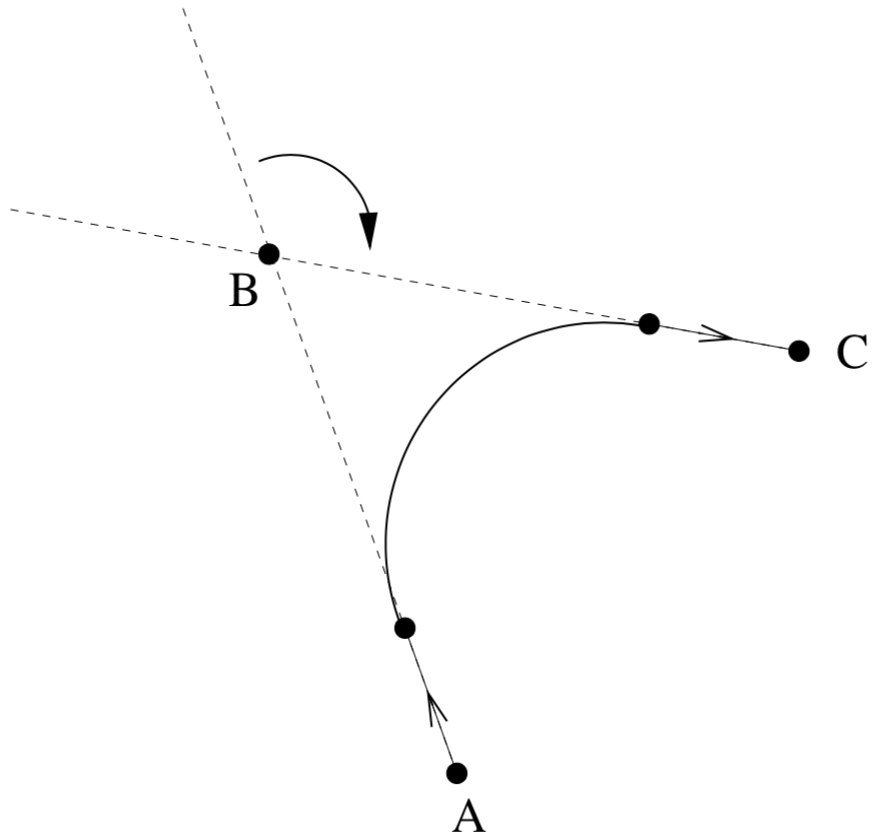
\includegraphics[height=2.55in]{fig631}
  \caption{Geometrical significance of the parameters for the {\em arc}
type code.}
\end{figure}
